% !TeX program = xelatex
% 编译：xelatex 12-函数的正交分解.tex（VS Code 的 LaTeX Workshop 会读上一行，自动用 xelatex）
% 来源：2022 浙江大学《信号与系统》胡浩基老师，函数的正交分解、函数的正交分解例子（PCA）。PCA 部分的幻灯片取自于慧敏教授《信号与系统》课件。
% 体例：内积 → 正交函数族 → 按正交函数族分解 → 标准正交基 → 用正交基重新推导傅里叶级数复数形式 → 其他正交基（哈尔小波、勒让德多项式）→ 收敛性 → 施密特正交化 → 主成分分析。
% 哈尔小波第三排按视频中的勘误画法；勒让德多项式、|x| 的部分和曲线：用 Python 计算后取样，直接写成 TikZ 坐标。
\documentclass[UTF8,a4paper,11pt]{ctexart}
\usepackage{amsmath,amssymb}
\usepackage{geometry}
\geometry{margin=2.4cm}
\usepackage{xcolor}
\usepackage{mdframed}
\usepackage{booktabs}
\usepackage{needspace}
\usepackage{array}
\usepackage{enumitem}
\usepackage{tikz}
\usetikzlibrary{arrows.meta,positioning,calc,patterns}
\usepackage{float}
\usepackage{fancyhdr}
% 页眉页脚清空，只在右下角保留页号（含首页）
\fancypagestyle{plain}{%
  \fancyhf{}%
  \fancyfoot[R]{\thepage}%
  \renewcommand{\headrulewidth}{0pt}%
  \renewcommand{\footrulewidth}{0pt}}
\usepackage[hidelinks,unicode,bookmarksnumbered,bookmarksopen=true,bookmarksopenlevel=2,pdftitle={函数的正交分解}]{hyperref}
\usepackage{bookmark}% XeTeX 下 hyperref 自带的大纲不生效，用 bookmark 宏包生成 PDF 书签（需编译两遍）

\setCJKmainfont{Songti SC}[BoldFont={Songti SC Bold}]
\setCJKsansfont{PingFang SC}

\newmdenv[backgroundcolor=blue!4,linecolor=blue!50!black,linewidth=1pt,innertopmargin=6pt,innerbottommargin=6pt]{rememberbox}
\newenvironment{remember}{\begin{rememberbox}\textbf{重点}\par\smallskip}{\end{rememberbox}}
\newmdenv[backgroundcolor=yellow!8,linecolor=orange!70!black,linewidth=1pt,innertopmargin=6pt,innerbottommargin=6pt]{notebox}
\newenvironment{note}{\begin{notebox}\textbf{说明}\par\smallskip}{\end{notebox}}

% ---------------------------------------------------------------- 画图用的小宏
% 坐标轴：\taxes[自变量名]{横轴起点}{横轴终点}{纵轴顶端}{纵轴底端}。原点标 0（放在左下，避开纵轴）。
\newcommand{\taxes}[5][t]{%
  \draw[->] (#2,0) -- (#3,0) node[right,font=\scriptsize] {$#1$};
  \draw[->] (0,#5) -- (0,#4);
  \node[anchor=north east,font=\tiny,gray!60!black,inner sep=1pt] at (0,-0.02) {$0$};}
% 横轴刻度 \xt{位置}{标签}（标在轴下方）、\xtu{位置}{标签}（标在轴上方）、纵轴刻度 \yt{位置}{标签}：刻度线 + 白底数字。
\newcommand{\xt}[2]{\draw (#1,0) -- (#1,-0.1) node[anchor=north,font=\tiny,gray!60!black,fill=white,inner sep=0.6pt] {$#2$};}
\newcommand{\xtu}[2]{\draw (#1,0) -- (#1,0.1) node[anchor=south,font=\tiny,gray!60!black,fill=white,inner sep=0.6pt] {$#2$};}
\newcommand{\yt}[2]{\draw (0,#1) -- (-0.1,#1) node[anchor=east,font=\tiny,gray!60!black,fill=white,inner sep=0.6pt] {$#2$};}
\tikzset{>=stealth,
  sig/.style={thick,blue!60!black},
  res/.style={thick,red!70!black},
  grn/.style={thick,green!45!black}}

% ---------------------------------------------------------------- 标题层级
\definecolor{secblue}{RGB}{31,78,121}
\definecolor{exorange}{RGB}{190,90,10}
\definecolor{ptteal}{RGB}{0,110,110}
\ctexset{
  section={format=\raggedright\Large\bfseries\color{secblue},
           beforeskip=3.2ex plus 1ex minus .5ex, afterskip=1.4ex,
           aftertitle={\par\nobreak\vspace{-1.1ex}\noindent\textcolor{secblue}{\rule{\linewidth}{0.8pt}}\par\nobreak\vspace{0.6ex}}},
  subsection={format=\raggedright\large\bfseries\color{secblue},
              beforeskip=2.4ex plus .8ex minus .4ex, afterskip=1.0ex}
}
% 例题标题：\example{标题}{结论}{附注}，附注一般留空。
\newcounter{ex}[section]
\newcommand{\example}[3]{%
  \refstepcounter{ex}\phantomsection
  \addcontentsline{toc}{subsubsection}{例 \theex\ #1（#2）}%
  \par\addvspace{1.6ex}\noindent
  {\setlength{\fboxsep}{3pt}%
   \colorbox{exorange}{\textcolor{white}{\textbf{例~\theex}}}\ %
   \textcolor{exorange}{\textbf{#1}}\ {\footnotesize\textcolor{gray!70!black}{#3}}%
   \hfill\colorbox{exorange!12}{\small\textcolor{exorange}{#2}}\par}%
  \nobreak\vskip0.6ex\relax\csname @afterheading\endcsname}
% 小标题（接着同一段往下写，不进大纲）：青色三角 + 粗体。
\newcommand{\point}[1]{\par\addvspace{1ex}\noindent\textcolor{ptteal}{$\blacktriangleright$\,\textbf{#1}}\ }

\title{函数的正交分解\\\large 浙江大学 2022《信号与系统》（胡浩基）第三章听课笔记}
\author{}
\date{}

\begin{document}
\pagestyle{plain}
\maketitle

%==================================================================
\section{从傅里叶级数说起}\label{sec:intro}
傅里叶级数能写成简单的形式、系数能简洁地算出来，核心原因是这个函数族
\[
\{1,\ \cos(\omega_0t),\ \cos(2\omega_0t),\ \dots,\ \sin(\omega_0t),\ \sin(2\omega_0t),\ \dots\}
\]
有一个性质：\textbf{任选两个相乘，在一个周期 $T_0=\frac{2\pi}{\omega_0}$ 上积分都为 $0$。}正因为有这个性质，系数才能写成
\[
B_0=\frac1{T_0}\int_{T_0}x(t)\,\mathrm{d}t,\quad
B_k=\frac2{T_0}\int_{T_0}x(t)\cos(k\omega_0t)\,\mathrm{d}t,\quad
C_k=\frac2{T_0}\int_{T_0}x(t)\sin(k\omega_0t)\,\mathrm{d}t,
\]
并有 $x(t)=B_0+\sum_{k=1}^{+\infty}B_k\cos(k\omega_0t)+\sum_{k=1}^{+\infty}C_k\sin(k\omega_0t)$。

把这个性质推广：一族函数 $\{e_i(t)\}_{i=1\sim+\infty}$，若任取两个 $e_i(t)$、$e_j(t)$（$i\ne j$）相乘并积分为 $0$：
\[
\int_a^b e_i(t)\,\overline{e_j(t)}\,\mathrm{d}t=0,
\]
就称这组函数为\textbf{正交函数族}。横线表示共轭；$\cos$、$\sin$ 是实函数，取共轭仍等于原来，所以傅里叶级数里看不出这个横线。

\begin{remember}
傅里叶级数的复数形式只需记两个公式，之后统一用这个形式：
\[
a_k=\frac1{T_0}\int_{T_0}x(t)\,e^{-jk\omega_0t}\,\mathrm{d}t,\qquad
x(t)=\sum_{k=-\infty}^{+\infty}a_k\,e^{jk\omega_0t}\qquad\Big(\omega_0=\frac{2\pi}{T_0}\Big).
\]
\end{remember}

下面先定义内积，再定义正交函数族、标准正交基，然后从正交基的角度重新推导傅里叶级数，最后看其他的正交基。

\begin{figure}[H]
\centering
\begin{tikzpicture}[x=1.15cm,y=1.1cm]
  \foreach \a/\b/\c in {0/0.7854/red!25,0.7854/1.5708/green!25,1.5708/2.3562/red!25,2.3562/3.9270/green!25,3.9270/4.7124/red!25,4.7124/5.4978/green!25,5.4978/6.2832/red!25}{%
    \fill[\c] plot[domain=\a:\b,samples=30] (\x,{cos(\x r)*cos(2*\x r)}) -- cycle;}
  \taxes{-0.3}{6.9}{1.4}{-1.4}
  \draw[blue!60!black,thin,dashed,domain=0:6.2832,samples=120] plot (\x,{cos(\x r)});
  \draw[green!45!black,thin,dashed,domain=0:6.2832,samples=120] plot (\x,{cos(2*\x r)});
  \draw[res,domain=0:6.2832,samples=200] plot (\x,{cos(\x r)*cos(2*\x r)});
  \xt{1.5708}{T_0/4}\xt{3.1416}{T_0/2}\xt{4.7124}{3T_0/4}\xt{6.2832}{T_0}
  \yt{1}{1}\yt{-1}{-1}
  \node[font=\footnotesize,blue!60!black,anchor=west] at (6.35,1.0) {$\cos(\omega_0t)$};
  \node[font=\footnotesize,green!45!black,anchor=west] at (6.35,0.55) {$\cos(2\omega_0t)$};
  \node[font=\footnotesize,red!70!black,anchor=west] at (6.35,-0.6) {乘积};
\end{tikzpicture}
\caption{取 $\omega_0=1$（$T_0=2\pi$）。$\cos(\omega_0t)$ 与 $\cos(2\omega_0t)$（虚线）的乘积（红线）在一个周期内，红色的正面积与绿色的负面积正好抵消，积分为 $0$。}
\end{figure}

%==================================================================
\section{内积}\label{sec:ip}
\begin{remember}
\textbf{内积}(inner product)：若一个运算 $\langle\cdot,\cdot\rangle$ 满足以下 4 个性质，就把这个运算叫做内积。
\begin{enumerate}[nosep,label=\textcircled{\scriptsize\arabic*}]
\item 交换律（共轭对称）：$\langle x,y\rangle=\overline{\langle y,x\rangle}$（横线代表共轭）；
\item 齐次性：$\langle\lambda x,y\rangle=\lambda\langle x,y\rangle$；
\item 叠加性：$\langle x+y,z\rangle=\langle x,z\rangle+\langle y,z\rangle$；
\item 非负性：$\langle x,x\rangle\ge0$，当且仅当 $x=0$ 时等号成立，即 $\langle0,0\rangle=0$。
\end{enumerate}
\end{remember}
实数情况下共轭就是它本身，交换律就是普通的 $\langle x,y\rangle=\langle y,x\rangle$。

\point{性质推论：数从右边拿出来要取共轭。}由 \textcircled{\scriptsize 1}\textcircled{\scriptsize 2}，
\[
\langle x,\lambda y\rangle=\overline{\langle\lambda y,x\rangle}=\overline{\lambda\langle y,x\rangle}=\overline{\lambda}\;\overline{\langle y,x\rangle}=\overline{\lambda}\,\langle x,y\rangle ;
\]
同理 $\langle x,y+z\rangle=\langle x,y\rangle+\langle x,z\rangle$。数从左边拿出来不变，从右边拿出来要加共轭。第 \ref{sec:gs} 节会用到。

\subsection{例一：函数的内积}
\begin{remember}
定义
\[
\langle x(t),y(t)\rangle=\int_a^b x(t)\,\overline{y(t)}\,\mathrm{d}t
\]
是内积。
\end{remember}
逐条验证 4 个性质：
\begin{enumerate}[nosep,label=\textcircled{\scriptsize\arabic*}]
\item 交换律：$\langle y,x\rangle=\int_a^b y(t)\,\overline{x(t)}\,\mathrm{d}t$，取共轭得 $\overline{\langle y,x\rangle}=\int_a^b\overline{y(t)}\,x(t)\,\mathrm{d}t=\int_a^b x(t)\,\overline{y(t)}\,\mathrm{d}t=\langle x,y\rangle$。
\item 齐次性：$\langle\lambda x,y\rangle=\int_a^b\lambda x(t)\,\overline{y(t)}\,\mathrm{d}t$，把常数 $\lambda$ 提到积分外，等于 $\lambda\langle x,y\rangle$。
\item 叠加性：由积分的叠加性，
\[
\langle x+y,z\rangle=\int_a^b\big(x(t)+y(t)\big)\overline{z(t)}\,\mathrm{d}t=\int_a^b x(t)\overline{z(t)}\,\mathrm{d}t+\int_a^b y(t)\overline{z(t)}\,\mathrm{d}t=\langle x,z\rangle+\langle y,z\rangle .
\]
\item 非负性：$\langle x,x\rangle=\int_a^b x(t)\,\overline{x(t)}\,\mathrm{d}t=\int_a^b|x(t)|^2\,\mathrm{d}t\ge0$（$x\overline{x}$ 是模的平方）。若 $x(t)$ 在 $[a,b]$ 内有一小段不为 $0$，积分一定大于 $0$；只有 $x(t)$ 在 $[a,b]$ 上为 $0$ 时积分才为 $0$。
\end{enumerate}

\point{只在有限个点上不为 $0$ 怎么办？}这时 $\int_a^b|x(t)|^2\,\mathrm{d}t=0$，但 $x(t)$ 似乎不是 $0$。按勒贝格对两个函数相等的定义（「冲激函数的性质」中的定义三），只在有限个点上与 $0$ 不同的函数就\textbf{等于} $0$，所以没有矛盾。

\subsection{例二：序列的内积}
\begin{remember}
定义
\[
\langle x[n],y[n]\rangle=\sum_{k=k_1}^{k_2}x[k]\,\overline{y[k]}
\]
也是内积。
\end{remember}
验证方法与例一相同，把积分换成求和：交换律、齐次性、叠加性都来自求和的性质；非负性 $\langle x,x\rangle=\sum_{k=k_1}^{k_2}|x[k]|^2\ge0$，等号当且仅当每个 $x[k]=0$。

%==================================================================
\section{正交函数族}\label{sec:orth}
\begin{remember}
\textbf{正交函数族}（正交基函数，orthogonal basis function）：若函数族 $\{e_1,e_2,\dots,e_N,\dots\}=\{e_k\}_{k=1\sim+\infty}$ 满足
\begin{enumerate}[nosep,label=\textcircled{\scriptsize\arabic*}]
\item $\forall k$，有 $\langle e_k,e_k\rangle>0$；
\item $\forall k_1\ne k_2$，有 $\langle e_{k_1},e_{k_2}\rangle=0$，
\end{enumerate}
则称 $\{e_k\}_{k=1\sim+\infty}$ 是正交函数族。
\end{remember}
条件 \textcircled{\scriptsize 1}：每个 $e_k$ 自己与自己的内积大于 $0$，也就是每个 $e_k$ 都不等于 $0$。条件 \textcircled{\scriptsize 2}：两个不同的函数做内积恒为 $0$。

\point{例。}$\{1,\cos(\omega_0t),\cos(2\omega_0t),\dots,\sin(\omega_0t),\sin(2\omega_0t),\dots\}$ 是正交函数族，其内积定义为
\[
\langle e_{k_1}(t),e_{k_2}(t)\rangle=\int_{T_0}e_{k_1}(t)\,\overline{e_{k_2}(t)}\,\mathrm{d}t ,
\]
即任取其中两个函数，在一个周期 $T_0$ 内积分。

\begin{note}
说一组函数正交，总是针对某个内积的定义说的。换一种内积（例如换积分区间），同一组函数不一定还正交。
\end{note}

%==================================================================
\section{把信号分解为正交函数族的线性叠加}\label{sec:dec}
设 $\{e_k(t)\}_{k=1\sim+\infty}$ 是正交函数族，假设
\[
x(t)=a_1e_1(t)+a_2e_2(t)+\cdots=\sum_{u=1}^{+\infty}a_ue_u(t),
\]
求 $a_k$。下标换成 $u$：要把 $k$ 留给待求的那一项，以免混淆（这个技巧前面用过多次）。

\point{求 $a_k$：两边与 $e_k(t)$ 做内积。}
\begin{align*}
\langle x(t),e_k(t)\rangle
&=\Big\langle\sum_{u=1}^{+\infty}a_ue_u(t),\,e_k(t)\Big\rangle\\
&=\sum_{u=1}^{+\infty}\big\langle a_ue_u(t),\,e_k(t)\big\rangle&&\text{（叠加性：求和号拿到外面）}\\
&=\sum_{u=1}^{+\infty}a_u\big\langle e_u(t),\,e_k(t)\big\rangle&&\text{（齐次性：$a_u$ 拿到外面）}\\
&=a_k\,\langle e_k(t),e_k(t)\rangle&&\text{（正交：只有 $u=k$ 的一项不为 $0$）}.
\end{align*}
由条件 \textcircled{\scriptsize 1}，$\langle e_k,e_k\rangle>0$，可以除过去：
\begin{remember}
正交函数族下的系数：
\[
a_k=\frac{\langle x(t),e_k(t)\rangle}{\langle e_k(t),e_k(t)\rangle}.
\]
\end{remember}
每个系数只要做一次内积就能单独算出来，不用解联立方程。这就是正交带来的好处。（叠加性对有限项成立；对无穷多项交换求和与内积，还要求级数收敛，见第 \ref{sec:conv} 节。）

\begin{figure}[H]
\centering
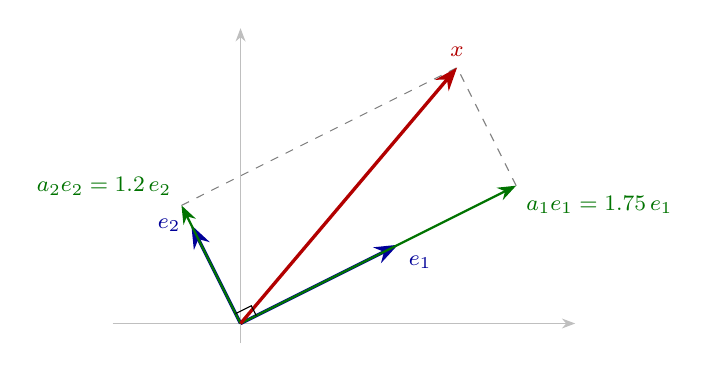
\begin{tikzpicture}[scale=1.25,>=Stealth]
  \draw[gray!50,->] (-1.3,0) -- (3.4,0);
  \draw[gray!50,->] (0,-0.2) -- (0,3.0);
  \draw[dashed,gray] (2.8,1.4) -- (2.2,2.6) -- (-0.6,1.2);
  \draw[very thick,->,blue!60!black] (0,0) -- (1.6,0.8) node[below right,font=\footnotesize] {$e_1$};
  \draw[very thick,->,blue!60!black] (0,0) -- (-0.5,1.0) node[left,font=\footnotesize] {$e_2$};
  \draw[thick,->,green!45!black] (0,0) -- (2.8,1.4) node[below right,font=\footnotesize] {$a_1e_1=1.75\,e_1$};
  \draw[thick,->,green!45!black] (0,0) -- (-0.6,1.2) node[above left,font=\footnotesize] {$a_2e_2=1.2\,e_2$};
  \draw[very thick,->,red!70!black] (0,0) -- (2.2,2.6) node[above,font=\footnotesize] {$x$};
  \draw (0.16,0.08) -- (0.11,0.18) -- (-0.05,0.10);
\end{tikzpicture}
\caption{二维的类比：$e_1=(1.6,0.8)$、$e_2=(-0.5,1.0)$ 互相垂直（内积为 $0$）。$x=(2.2,2.6)$ 的系数 $a_1=\frac{\langle x,e_1\rangle}{\langle e_1,e_1\rangle}=\frac{5.6}{3.2}=1.75$，$a_2=\frac{\langle x,e_2\rangle}{\langle e_2,e_2\rangle}=\frac{1.5}{1.25}=1.2$，两个分量合起来正好是 $x$。}
\end{figure}

%==================================================================
\section{标准正交基}\label{sec:onb}
\begin{remember}
\textbf{标准正交基函数}(orthonormal basis function)：若函数族 $\{e_k\}_{k=1\sim+\infty}$ 满足
\begin{enumerate}[nosep,label=\textcircled{\scriptsize\arabic*}]
\item $\forall k$，有 $\langle e_k,e_k\rangle=1$；
\item $\forall k_1\ne k_2$，有 $\langle e_{k_1},e_{k_2}\rangle=0$，
\end{enumerate}
则称它是标准正交基。
\end{remember}
orthonormal 是 orthogonal 与 normal 两个词合在一起。与正交基相比，只是把条件 \textcircled{\scriptsize 1} 的「$>0$」换成了「$=1$」。把自己与自己的内积看作这个基的长度，标准正交基就是把每个基的长度归一化(normalize)到 $1$。

\subsection{正交基的标准化}
把正交基变为标准正交基，叫做正交基的标准化：
\begin{remember}
正交基的标准化公式：
\[
e_k'=\frac{e_k}{\sqrt{\langle e_k,e_k\rangle}} .
\]
\end{remember}
验证：$\sqrt{\langle e_k,e_k\rangle}$ 是正实数，由齐次性和它的推论，
$\langle e_k',e_k'\rangle=\dfrac{\langle e_k,e_k\rangle}{\sqrt{\langle e_k,e_k\rangle}\cdot\sqrt{\langle e_k,e_k\rangle}}=1$；
不同的 $e_k'$ 之间的内积只是原来的 $0$ 乘一个数，仍为 $0$。

\example{把傅里叶级数的正交基标准化}{除以各自的长度}{}
\textbf{题目}：如何把 $\{1,\cos(k\omega_0t),\sin(k\omega_0t)\}$ 变成标准正交基？（内积为在一个周期 $T_0$ 上积分。）

\textbf{解}：
\[
1\longrightarrow\frac{1}{\sqrt{T_0}},\qquad
\cos(k\omega_0t)\longrightarrow\sqrt{\frac{2}{T_0}}\cos(k\omega_0t),\qquad
\sin(k\omega_0t)\longrightarrow\sqrt{\frac{2}{T_0}}\sin(k\omega_0t).
\]
验证前两个（都是实函数，共轭等于本身）：
\begin{gather*}
\Big\langle\frac1{\sqrt{T_0}},\frac1{\sqrt{T_0}}\Big\rangle=\int_0^{T_0}\frac1{\sqrt{T_0}}\cdot\frac1{\sqrt{T_0}}\,\mathrm{d}t=\frac1{T_0}\cdot T_0=1,\\
\Big\langle\sqrt{\tfrac2{T_0}}\cos(k\omega_0t),\sqrt{\tfrac2{T_0}}\cos(k\omega_0t)\Big\rangle=\frac2{T_0}\int_0^{T_0}\cos^2(k\omega_0t)\,\mathrm{d}t=\frac2{T_0}\cdot\frac{T_0}2=1 .
\end{gather*}
这里用到 $\int_0^{T_0}\cos^2(k\omega_0t)\,\mathrm{d}t=\frac{T_0}{2}$。$\sin$ 的验证相同。

\subsection{标准正交基下的分解公式}
若 $\{e_k\}$ 是标准正交基，第 \ref{sec:dec} 节的推导完全一样，只是最后一步 $\langle e_k,e_k\rangle=1$，分母直接去掉：
\begin{remember}
（只对标准正交基成立）
\[
a_k=\langle x(t),e_k(t)\rangle,\qquad
x(t)=\sum_{k=1}^{+\infty}a_ke_k(t)=\sum_{k=1}^{+\infty}\langle x(t),e_k(t)\rangle\,e_k(t).
\]
\end{remember}

%==================================================================
\section{从正交基的角度再次理解傅里叶级数（复数形式）}\label{sec:fs}
复数形式的两个公式：
\[
a_k=\frac1{T_0}\int_{T_0}x(t)\,e^{-jk\omega_0t}\,\mathrm{d}t,\qquad
x(t)=\sum_{k=-\infty}^{+\infty}a_k\,e^{jk\omega_0t}.
\]

\subsection{第一步：\texorpdfstring{$\{e^{jk\omega_0t}\}$}{exp(jkω0t)} 是正交基}
\begin{remember}
$\{e^{jk\omega_0t}\}_{k=-\infty\sim+\infty}$（$k$ 取整数）是正交基，内积为 $\langle x,y\rangle=\int_{T_0}x(t)\overline{y(t)}\,\mathrm{d}t$，且
\[
\langle e^{jk\omega_0t},e^{jk\omega_0t}\rangle=T_0,\qquad
\langle e^{jk_1\omega_0t},e^{jk_2\omega_0t}\rangle=0\quad(k_1\ne k_2).
\]
\end{remember}

\point{两个 $k$ 相同。}
\[
\langle e^{jk\omega_0t},e^{jk\omega_0t}\rangle=\int_{T_0}e^{jk\omega_0t}\,\overline{e^{jk\omega_0t}}\,\mathrm{d}t
=\int_0^{T_0}e^{jk\omega_0t}\cdot e^{-jk\omega_0t}\,\mathrm{d}t=\int_0^{T_0}1\,\mathrm{d}t=T_0 .
\]
共轭的分解动作：$e^{jk\omega_0t}=\cos(k\omega_0t)+j\sin(k\omega_0t)$，取共轭把 $+j$ 变成 $-j$，即 $\overline{e^{jk\omega_0t}}=\cos(k\omega_0t)-j\sin(k\omega_0t)=e^{-jk\omega_0t}$。两个指数相乘抵消成 $e^0=1$。

\point{两个 $k$ 不同（$k_1\ne k_2$）。}
\begin{align*}
\langle e^{jk_1\omega_0t},e^{jk_2\omega_0t}\rangle
&=\int_{T_0}e^{jk_1\omega_0t}\,\overline{e^{jk_2\omega_0t}}\,\mathrm{d}t
=\int_0^{T_0}e^{j(k_1-k_2)\omega_0t}\,\mathrm{d}t\\
&=\frac{1}{j(k_1-k_2)\omega_0}\,e^{j(k_1-k_2)\omega_0t}\Big|_{t=0}^{T_0}
=\frac{1}{j(k_1-k_2)\omega_0}\Big(e^{j(k_1-k_2)\omega_0T_0}-1\Big).
\end{align*}
$k_1-k_2\ne0$，所以可以这样积分。$\omega_0T_0=2\pi$，$k_1-k_2$ 是整数，而对任意整数 $k$，
\[
e^{j2\pi k}=\cos(2k\pi)+j\sin(2k\pi)=1+0=1,
\]
所以结果是 $\frac{1}{j(k_1-k_2)\omega_0}(1-1)=0$。

\subsection{第二步：推出系数公式}
设 $x(t)=\sum_{k=-\infty}^{+\infty}a_ke^{jk\omega_0t}$，两边与 $e^{jk\omega_0t}$ 做内积（下标换成 $u$）：
\begin{align*}
\langle x(t),e^{jk\omega_0t}\rangle
&=\Big\langle\sum_{u=-\infty}^{+\infty}a_ue^{ju\omega_0t},\,e^{jk\omega_0t}\Big\rangle
=\sum_{u=-\infty}^{+\infty}a_u\big\langle e^{ju\omega_0t},e^{jk\omega_0t}\big\rangle
=T_0\,a_k .
\end{align*}
$u\ne k$ 的项内积为 $0$，$u=k$ 的项内积为 $T_0$。因此
\begin{remember}
傅里叶级数复数形式的系数：
\[
a_k=\frac1{T_0}\langle x(t),e^{jk\omega_0t}\rangle
=\frac1{T_0}\int_{T_0}x(t)\,\overline{e^{jk\omega_0t}}\,\mathrm{d}t
=\frac1{T_0}\int_{T_0}x(t)\,e^{-jk\omega_0t}\,\mathrm{d}t .
\]
\end{remember}
系数公式里的负号来自内积定义中的共轭；前面的 $\frac1{T_0}$ 来自 $\langle e^{jk\omega_0t},e^{jk\omega_0t}\rangle=T_0$——这组基是正交基，不是标准正交基。用内积来推导，对傅里叶级数的理解会更深一层。

%==================================================================
\section{其他的正交基函数}\label{sec:other}
傅里叶是第一个把一个信号分解为一组正交基的线性叠加的人。他用的这组正交基是常数、$\cos$ 和 $\sin$。在他之后，很多人做了同样的事：只要能造出另外一组正交基，用上面这套理论，就能把信号分解为另外一组正交基函数的叠加。

\subsection{哈尔小波}\label{sub:haar}
1909 年，哈尔(Haar)造出了另一组正交基，叫做哈尔小波(Haar wavelet)。记单位方波和基本小波为
\[
\varphi(t)=\begin{cases}1,&0\le t<1\\0,&\text{其他}\end{cases},\qquad
\psi(t)=\begin{cases}1,&0\le t<\frac12\\-1,&\frac12\le t<1\\0,&\text{其他}\end{cases}.
\]
\begin{remember}
哈尔小波正交基（$n$、$m$ 取所有整数）：
\begin{enumerate}[nosep,label=\textcircled{\scriptsize\arabic*}]
\item 第一排：$\varphi(t-n)$，每个单位区间 $[n,n+1)$ 上一个高为 $1$ 的方波；
\item 第二排：$\psi(t-n)$，在 $[n,n+1)$ 上前一半为 $1$、后一半为 $-1$；
\item 第三排：$\psi(2t-m)$，宽度缩为 $\frac12$，每个单位区间里有\textbf{两个}，例如 $[0,\frac12)$ 与 $[\frac12,1)$ 各一个；
\item 第四排：$\psi(4t-m)$，宽度 $\frac14$，每个单位区间里有四个；以此类推，第 $j+2$ 排是 $\psi(2^jt-m)$。
\end{enumerate}
\end{remember}

\begin{figure}[H]
\centering
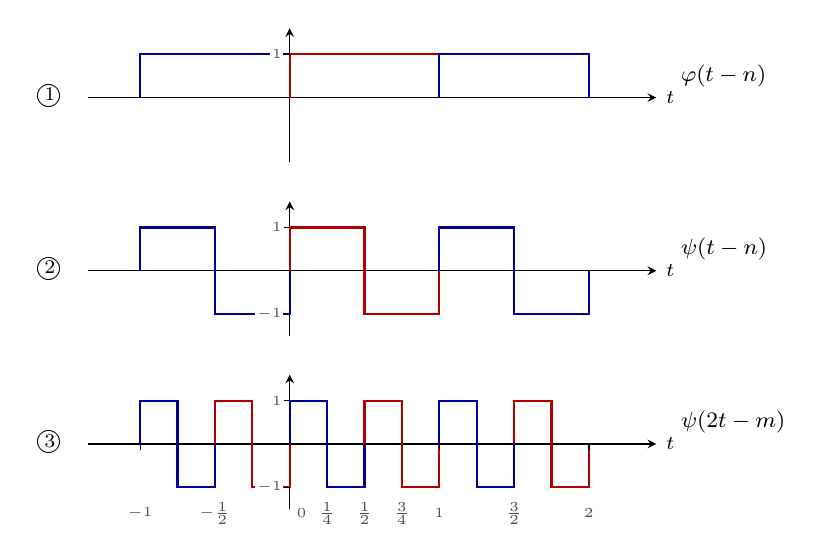
\begin{tikzpicture}[x=1.9cm,y=0.55cm]
  \newcommand{\row}[2]{\node[anchor=east,font=\footnotesize] at (-1.45,#1) {#2};
    \draw[->] (-1.35,#1) -- (2.45,#1) node[right,font=\scriptsize] {$t$};
    \draw[->] (0,#1-1.5) -- (0,#1+1.6);}
  % 第一排
  \row{0}{\textcircled{\scriptsize 1}}
  \draw[thick,blue!60!black] (-1,0) -- (-1,1) -- (0,1) -- (0,0);
  \draw[thick,red!70!black] (0,0) -- (0,1) -- (1,1) -- (1,0);
  \draw[thick,blue!60!black] (1,0) -- (1,1) -- (2,1) -- (2,0);
  % 第二排
  \row{-4}{\textcircled{\scriptsize 2}}
  \draw[thick,blue!60!black] (-1,-4) -- (-1,-3) -- (-0.5,-3) -- (-0.5,-5) -- (0,-5) -- (0,-4);
  \draw[thick,red!70!black] (0,-4) -- (0,-3) -- (0.5,-3) -- (0.5,-5) -- (1,-5) -- (1,-4);
  \draw[thick,blue!60!black] (1,-4) -- (1,-3) -- (1.5,-3) -- (1.5,-5) -- (2,-5) -- (2,-4);
  % 第三排
  \row{-8}{\textcircled{\scriptsize 3}}
  \foreach \s/\c in {-1/blue!60!black,-0.5/red!70!black,0/blue!60!black,0.5/red!70!black,1/blue!60!black,1.5/red!70!black}{%
    \draw[thick,\c] (\s,-8) -- (\s,-7) -- (\s+0.25,-7) -- (\s+0.25,-9) -- (\s+0.5,-9) -- (\s+0.5,-8);}
  % 刻度
  \foreach \p in {-1,1,2}{\draw (\p,-8) -- (\p,-8.15);}
  \node[font=\tiny,gray!60!black,fill=white,inner sep=0.6pt] at (-1,-9.6) {$-1$};
  \node[font=\tiny,gray!60!black,fill=white,inner sep=0.6pt] at (-0.5,-9.6) {$-\frac12$};
  \node[font=\tiny,gray!60!black,fill=white,inner sep=0.6pt] at (0.08,-9.6) {$0$};
  \node[font=\tiny,gray!60!black,fill=white,inner sep=0.6pt] at (0.25,-9.6) {$\frac14$};
  \node[font=\tiny,gray!60!black,fill=white,inner sep=0.6pt] at (0.5,-9.6) {$\frac12$};
  \node[font=\tiny,gray!60!black,fill=white,inner sep=0.6pt] at (0.75,-9.6) {$\frac34$};
  \node[font=\tiny,gray!60!black,fill=white,inner sep=0.6pt] at (1,-9.6) {$1$};
  \node[font=\tiny,gray!60!black,fill=white,inner sep=0.6pt] at (1.5,-9.6) {$\frac32$};
  \node[font=\tiny,gray!60!black,fill=white,inner sep=0.6pt] at (2,-9.6) {$2$};
  \foreach \r in {0,-4,-8}{%
    \draw (0,\r+1) -- (-0.04,\r+1) node[anchor=east,font=\tiny,gray!60!black,fill=white,inner sep=0.6pt] {$1$};}
  \foreach \r in {-4,-8}{%
    \draw (0,\r-1) -- (-0.04,\r-1) node[anchor=east,font=\tiny,gray!60!black,fill=white,inner sep=0.6pt] {$-1$};}
  \node[font=\footnotesize,anchor=west] at (2.55,0.5) {$\varphi(t-n)$};
  \node[font=\footnotesize,anchor=west] at (2.55,-3.5) {$\psi(t-n)$};
  \node[font=\footnotesize,anchor=west] at (2.55,-7.5) {$\psi(2t-m)$};
\end{tikzpicture}
\caption{哈尔小波的前三排，画出 $[-1,2]$ 一段（向左右无限延伸）。红、蓝只用来区分相邻的不同函数：每一段方波或「上一下一」都是一个单独的基函数。第三排每个单位区间里有两个宽 $\frac12$ 的小波。}
\end{figure}

\point{为什么正交。}以第二排的 $\psi(t)$（在 $[0,1)$ 上）为例：
\begin{itemize}[nosep]
\item 与第一排：除了 $\varphi(t)$ 之外，第一排其他方波在 $[0,1)$ 上没有值，乘起来积分为 $0$；与 $\varphi(t)$ 相乘，前一半是 $+1$、后一半是 $-1$，正负抵消，积分也为 $0$。
\item 与第二排其他函数：不重叠，积分为 $0$。
\end{itemize}
第三排同理：每个 $\psi(2t-m)$ 落在第一、二排某个函数的「平的一段」上（值为常数），自己又正负各一半，相乘积分为 $0$；第三排内部互不重叠。往下每一排都这样。

\point{为什么叫小波。}小波的意思是：只在时间轴上的一段有值，在其他地方都等于 $0$。$\sin$、$\cos$ 从 $-\infty$ 到 $+\infty$ 都有值，所以傅里叶级数的基不是小波；哈尔造出的这组正交基是小波。

信号分解为哈尔小波的方法与前面完全一样：对每个基函数算内积，再按 $a_k=\frac{\langle x,e_k\rangle}{\langle e_k,e_k\rangle}$ 求系数。注意这组基不是标准正交的：$\langle\varphi,\varphi\rangle=\langle\psi,\psi\rangle=1$，但第三排 $\langle\psi(2t),\psi(2t)\rangle=\frac12$，一般地 $\langle\psi(2^jt-m),\psi(2^jt-m)\rangle=2^{-j}$；标准化后为 $2^{j/2}\psi(2^jt-m)$。

\begin{note}
\textbf{易错：第三排不能把两个小波画成一个函数。}若把 $[0,1)$ 上的 $\psi(2t)$ 与 $\psi(2t-1)$ 合成一个函数 $w(t)$（四段依次为 $1,-1,1,-1$），$w$ 与第一、二排仍然正交，但这组函数不再完备，有的函数无论取多少项都逼近不了。例：$g(t)$ 在 $[0,\frac14)$ 上为 $1$，其他地方为 $0$。
\begin{itemize}[nosep]
\item 正确的基：$g=\frac14\varphi(t)+\frac14\psi(t)+\frac12\psi(2t)$，四段依次是 $\frac14+\frac14+\frac12=1$、$\frac14+\frac14-\frac12=0$、$\frac14-\frac14=0$、$0$，成立。
\item 合成后的基：设 $g$ 在 $[0,1)$ 四段上的平均值由 $c_1\varphi+c_2\psi+c_3w$ 给出，要求 $c_1+c_2+c_3=1$、$c_1+c_2-c_3=0$ 推出 $c_3=\frac12$，又要求 $c_1-c_2+c_3=0$、$c_1-c_2-c_3=0$ 推出 $c_3=0$，矛盾。第四排及以后的函数在每个 $\frac14$ 小段上积分都为 $0$，改变不了这四个平均值，所以再加多少项也不行。
\end{itemize}
\end{note}

\subsection{勒让德多项式}\label{sub:legendre}
勒让德(Legendre)是法国数学家。勒让德多项式(Legendre polynomials)：
\begin{remember}
勒让德多项式（罗德里格斯公式）：
\[
P_n(x)=\frac{1}{2^n\,n!}\,\frac{\mathrm{d}^n}{\mathrm{d}x^n}\big[(x^2-1)^n\big],\qquad n=0,1,2,\dots
\]
勒让德多项式的正交性：
\[
\int_{-1}^{1}\big[P_n(x)\big]^2\,\mathrm{d}x=\frac{2}{2n+1},\qquad
\int_{-1}^{1}P_m(x)\,P_n(x)\,\mathrm{d}x=0\quad(m\ne n).
\]
\end{remember}
正交性的证明可以查阅数学分析或数学物理方法的教材，这里不展开。

\point{前几个。}$P_0(x)=1$，$P_1(x)=x$，$P_3(x)=\frac{5x^3-3x}{2}$。以 $P_2$ 为例按公式算：
\[
P_2(x)=\frac{1}{2^2\cdot2!}\,\frac{\mathrm{d}^2}{\mathrm{d}x^2}\big(x^4-2x^2+1\big)=\frac18\big(12x^2-4\big)=\frac{3x^2-1}{2}.
\]

\begin{figure}[H]
\centering
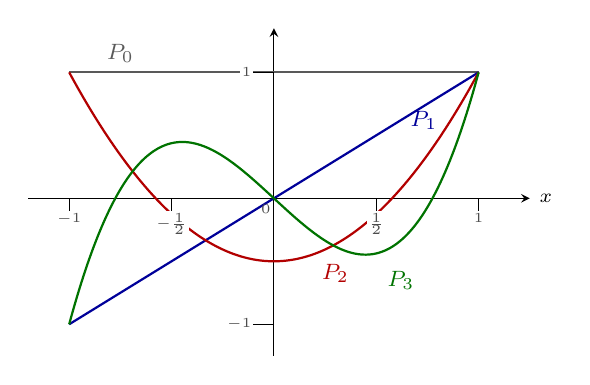
\begin{tikzpicture}[x=2.6cm,y=1.6cm]
  \draw[->] (-1.2,0) -- (1.25,0) node[right,font=\scriptsize] {$x$};
  \draw[->] (0,-1.25) -- (0,1.35);
  \draw[thick,gray!70!black] plot coordinates {(-1.0000,1.0000) (-0.9900,1.0000) (-0.9800,1.0000) (-0.9700,1.0000) (-0.9600,1.0000) (-0.9500,1.0000) (-0.9400,1.0000) (-0.9300,1.0000) (-0.9200,1.0000) (-0.9100,1.0000) (-0.9000,1.0000) (-0.8900,1.0000) (-0.8800,1.0000) (-0.8700,1.0000) (-0.8600,1.0000) (-0.8500,1.0000) (-0.8400,1.0000) (-0.8300,1.0000) (-0.8200,1.0000) (-0.8100,1.0000) (-0.8000,1.0000) (-0.7900,1.0000) (-0.7800,1.0000) (-0.7700,1.0000) (-0.7600,1.0000) (-0.7500,1.0000) (-0.7400,1.0000) (-0.7300,1.0000) (-0.7200,1.0000) (-0.7100,1.0000) (-0.7000,1.0000) (-0.6900,1.0000) (-0.6800,1.0000) (-0.6700,1.0000) (-0.6600,1.0000) (-0.6500,1.0000) (-0.6400,1.0000) (-0.6300,1.0000) (-0.6200,1.0000) (-0.6100,1.0000) (-0.6000,1.0000) (-0.5900,1.0000) (-0.5800,1.0000) (-0.5700,1.0000) (-0.5600,1.0000) (-0.5500,1.0000) (-0.5400,1.0000) (-0.5300,1.0000) (-0.5200,1.0000) (-0.5100,1.0000) (-0.5000,1.0000) (-0.4900,1.0000) (-0.4800,1.0000) (-0.4700,1.0000) (-0.4600,1.0000) (-0.4500,1.0000) (-0.4400,1.0000) (-0.4300,1.0000) (-0.4200,1.0000) (-0.4100,1.0000) (-0.4000,1.0000) (-0.3900,1.0000) (-0.3800,1.0000) (-0.3700,1.0000) (-0.3600,1.0000) (-0.3500,1.0000) (-0.3400,1.0000) (-0.3300,1.0000) (-0.3200,1.0000) (-0.3100,1.0000) (-0.3000,1.0000) (-0.2900,1.0000) (-0.2800,1.0000) (-0.2700,1.0000) (-0.2600,1.0000) (-0.2500,1.0000) (-0.2400,1.0000) (-0.2300,1.0000) (-0.2200,1.0000) (-0.2100,1.0000) (-0.2000,1.0000) (-0.1900,1.0000) (-0.1800,1.0000) (-0.1700,1.0000) (-0.1600,1.0000) (-0.1500,1.0000) (-0.1400,1.0000) (-0.1300,1.0000) (-0.1200,1.0000) (-0.1100,1.0000) (-0.1000,1.0000) (-0.0900,1.0000) (-0.0800,1.0000) (-0.0700,1.0000) (-0.0600,1.0000) (-0.0500,1.0000) (-0.0400,1.0000) (-0.0300,1.0000) (-0.0200,1.0000) (-0.0100,1.0000) (0.0000,1.0000) (0.0100,1.0000) (0.0200,1.0000) (0.0300,1.0000) (0.0400,1.0000) (0.0500,1.0000) (0.0600,1.0000) (0.0700,1.0000) (0.0800,1.0000) (0.0900,1.0000) (0.1000,1.0000) (0.1100,1.0000) (0.1200,1.0000) (0.1300,1.0000) (0.1400,1.0000) (0.1500,1.0000) (0.1600,1.0000) (0.1700,1.0000) (0.1800,1.0000) (0.1900,1.0000) (0.2000,1.0000) (0.2100,1.0000) (0.2200,1.0000) (0.2300,1.0000) (0.2400,1.0000) (0.2500,1.0000) (0.2600,1.0000) (0.2700,1.0000) (0.2800,1.0000) (0.2900,1.0000) (0.3000,1.0000) (0.3100,1.0000) (0.3200,1.0000) (0.3300,1.0000) (0.3400,1.0000) (0.3500,1.0000) (0.3600,1.0000) (0.3700,1.0000) (0.3800,1.0000) (0.3900,1.0000) (0.4000,1.0000) (0.4100,1.0000) (0.4200,1.0000) (0.4300,1.0000) (0.4400,1.0000) (0.4500,1.0000) (0.4600,1.0000) (0.4700,1.0000) (0.4800,1.0000) (0.4900,1.0000) (0.5000,1.0000) (0.5100,1.0000) (0.5200,1.0000) (0.5300,1.0000) (0.5400,1.0000) (0.5500,1.0000) (0.5600,1.0000) (0.5700,1.0000) (0.5800,1.0000) (0.5900,1.0000) (0.6000,1.0000) (0.6100,1.0000) (0.6200,1.0000) (0.6300,1.0000) (0.6400,1.0000) (0.6500,1.0000) (0.6600,1.0000) (0.6700,1.0000) (0.6800,1.0000) (0.6900,1.0000) (0.7000,1.0000) (0.7100,1.0000) (0.7200,1.0000) (0.7300,1.0000) (0.7400,1.0000) (0.7500,1.0000) (0.7600,1.0000) (0.7700,1.0000) (0.7800,1.0000) (0.7900,1.0000) (0.8000,1.0000) (0.8100,1.0000) (0.8200,1.0000) (0.8300,1.0000) (0.8400,1.0000) (0.8500,1.0000) (0.8600,1.0000) (0.8700,1.0000) (0.8800,1.0000) (0.8900,1.0000) (0.9000,1.0000) (0.9100,1.0000) (0.9200,1.0000) (0.9300,1.0000) (0.9400,1.0000) (0.9500,1.0000) (0.9600,1.0000) (0.9700,1.0000) (0.9800,1.0000) (0.9900,1.0000) (1.0000,1.0000)};
  \draw[sig] plot coordinates {(-1.0000,-1.0000) (-0.9900,-0.9900) (-0.9800,-0.9800) (-0.9700,-0.9700) (-0.9600,-0.9600) (-0.9500,-0.9500) (-0.9400,-0.9400) (-0.9300,-0.9300) (-0.9200,-0.9200) (-0.9100,-0.9100) (-0.9000,-0.9000) (-0.8900,-0.8900) (-0.8800,-0.8800) (-0.8700,-0.8700) (-0.8600,-0.8600) (-0.8500,-0.8500) (-0.8400,-0.8400) (-0.8300,-0.8300) (-0.8200,-0.8200) (-0.8100,-0.8100) (-0.8000,-0.8000) (-0.7900,-0.7900) (-0.7800,-0.7800) (-0.7700,-0.7700) (-0.7600,-0.7600) (-0.7500,-0.7500) (-0.7400,-0.7400) (-0.7300,-0.7300) (-0.7200,-0.7200) (-0.7100,-0.7100) (-0.7000,-0.7000) (-0.6900,-0.6900) (-0.6800,-0.6800) (-0.6700,-0.6700) (-0.6600,-0.6600) (-0.6500,-0.6500) (-0.6400,-0.6400) (-0.6300,-0.6300) (-0.6200,-0.6200) (-0.6100,-0.6100) (-0.6000,-0.6000) (-0.5900,-0.5900) (-0.5800,-0.5800) (-0.5700,-0.5700) (-0.5600,-0.5600) (-0.5500,-0.5500) (-0.5400,-0.5400) (-0.5300,-0.5300) (-0.5200,-0.5200) (-0.5100,-0.5100) (-0.5000,-0.5000) (-0.4900,-0.4900) (-0.4800,-0.4800) (-0.4700,-0.4700) (-0.4600,-0.4600) (-0.4500,-0.4500) (-0.4400,-0.4400) (-0.4300,-0.4300) (-0.4200,-0.4200) (-0.4100,-0.4100) (-0.4000,-0.4000) (-0.3900,-0.3900) (-0.3800,-0.3800) (-0.3700,-0.3700) (-0.3600,-0.3600) (-0.3500,-0.3500) (-0.3400,-0.3400) (-0.3300,-0.3300) (-0.3200,-0.3200) (-0.3100,-0.3100) (-0.3000,-0.3000) (-0.2900,-0.2900) (-0.2800,-0.2800) (-0.2700,-0.2700) (-0.2600,-0.2600) (-0.2500,-0.2500) (-0.2400,-0.2400) (-0.2300,-0.2300) (-0.2200,-0.2200) (-0.2100,-0.2100) (-0.2000,-0.2000) (-0.1900,-0.1900) (-0.1800,-0.1800) (-0.1700,-0.1700) (-0.1600,-0.1600) (-0.1500,-0.1500) (-0.1400,-0.1400) (-0.1300,-0.1300) (-0.1200,-0.1200) (-0.1100,-0.1100) (-0.1000,-0.1000) (-0.0900,-0.0900) (-0.0800,-0.0800) (-0.0700,-0.0700) (-0.0600,-0.0600) (-0.0500,-0.0500) (-0.0400,-0.0400) (-0.0300,-0.0300) (-0.0200,-0.0200) (-0.0100,-0.0100) (0.0000,0.0000) (0.0100,0.0100) (0.0200,0.0200) (0.0300,0.0300) (0.0400,0.0400) (0.0500,0.0500) (0.0600,0.0600) (0.0700,0.0700) (0.0800,0.0800) (0.0900,0.0900) (0.1000,0.1000) (0.1100,0.1100) (0.1200,0.1200) (0.1300,0.1300) (0.1400,0.1400) (0.1500,0.1500) (0.1600,0.1600) (0.1700,0.1700) (0.1800,0.1800) (0.1900,0.1900) (0.2000,0.2000) (0.2100,0.2100) (0.2200,0.2200) (0.2300,0.2300) (0.2400,0.2400) (0.2500,0.2500) (0.2600,0.2600) (0.2700,0.2700) (0.2800,0.2800) (0.2900,0.2900) (0.3000,0.3000) (0.3100,0.3100) (0.3200,0.3200) (0.3300,0.3300) (0.3400,0.3400) (0.3500,0.3500) (0.3600,0.3600) (0.3700,0.3700) (0.3800,0.3800) (0.3900,0.3900) (0.4000,0.4000) (0.4100,0.4100) (0.4200,0.4200) (0.4300,0.4300) (0.4400,0.4400) (0.4500,0.4500) (0.4600,0.4600) (0.4700,0.4700) (0.4800,0.4800) (0.4900,0.4900) (0.5000,0.5000) (0.5100,0.5100) (0.5200,0.5200) (0.5300,0.5300) (0.5400,0.5400) (0.5500,0.5500) (0.5600,0.5600) (0.5700,0.5700) (0.5800,0.5800) (0.5900,0.5900) (0.6000,0.6000) (0.6100,0.6100) (0.6200,0.6200) (0.6300,0.6300) (0.6400,0.6400) (0.6500,0.6500) (0.6600,0.6600) (0.6700,0.6700) (0.6800,0.6800) (0.6900,0.6900) (0.7000,0.7000) (0.7100,0.7100) (0.7200,0.7200) (0.7300,0.7300) (0.7400,0.7400) (0.7500,0.7500) (0.7600,0.7600) (0.7700,0.7700) (0.7800,0.7800) (0.7900,0.7900) (0.8000,0.8000) (0.8100,0.8100) (0.8200,0.8200) (0.8300,0.8300) (0.8400,0.8400) (0.8500,0.8500) (0.8600,0.8600) (0.8700,0.8700) (0.8800,0.8800) (0.8900,0.8900) (0.9000,0.9000) (0.9100,0.9100) (0.9200,0.9200) (0.9300,0.9300) (0.9400,0.9400) (0.9500,0.9500) (0.9600,0.9600) (0.9700,0.9700) (0.9800,0.9800) (0.9900,0.9900) (1.0000,1.0000)};
  \draw[res] plot coordinates {(-1.0000,1.0000) (-0.9900,0.9701) (-0.9800,0.9406) (-0.9700,0.9114) (-0.9600,0.8824) (-0.9500,0.8537) (-0.9400,0.8254) (-0.9300,0.7974) (-0.9200,0.7696) (-0.9100,0.7422) (-0.9000,0.7150) (-0.8900,0.6882) (-0.8800,0.6616) (-0.8700,0.6353) (-0.8600,0.6094) (-0.8500,0.5837) (-0.8400,0.5584) (-0.8300,0.5333) (-0.8200,0.5086) (-0.8100,0.4842) (-0.8000,0.4600) (-0.7900,0.4362) (-0.7800,0.4126) (-0.7700,0.3894) (-0.7600,0.3664) (-0.7500,0.3438) (-0.7400,0.3214) (-0.7300,0.2994) (-0.7200,0.2776) (-0.7100,0.2561) (-0.7000,0.2350) (-0.6900,0.2141) (-0.6800,0.1936) (-0.6700,0.1733) (-0.6600,0.1534) (-0.6500,0.1337) (-0.6400,0.1144) (-0.6300,0.0954) (-0.6200,0.0766) (-0.6100,0.0582) (-0.6000,0.0400) (-0.5900,0.0222) (-0.5800,0.0046) (-0.5700,-0.0126) (-0.5600,-0.0296) (-0.5500,-0.0462) (-0.5400,-0.0626) (-0.5300,-0.0786) (-0.5200,-0.0944) (-0.5100,-0.1099) (-0.5000,-0.1250) (-0.4900,-0.1399) (-0.4800,-0.1544) (-0.4700,-0.1687) (-0.4600,-0.1826) (-0.4500,-0.1963) (-0.4400,-0.2096) (-0.4300,-0.2227) (-0.4200,-0.2354) (-0.4100,-0.2478) (-0.4000,-0.2600) (-0.3900,-0.2719) (-0.3800,-0.2834) (-0.3700,-0.2947) (-0.3600,-0.3056) (-0.3500,-0.3163) (-0.3400,-0.3266) (-0.3300,-0.3367) (-0.3200,-0.3464) (-0.3100,-0.3559) (-0.3000,-0.3650) (-0.2900,-0.3738) (-0.2800,-0.3824) (-0.2700,-0.3906) (-0.2600,-0.3986) (-0.2500,-0.4062) (-0.2400,-0.4136) (-0.2300,-0.4207) (-0.2200,-0.4274) (-0.2100,-0.4339) (-0.2000,-0.4400) (-0.1900,-0.4459) (-0.1800,-0.4514) (-0.1700,-0.4567) (-0.1600,-0.4616) (-0.1500,-0.4662) (-0.1400,-0.4706) (-0.1300,-0.4747) (-0.1200,-0.4784) (-0.1100,-0.4819) (-0.1000,-0.4850) (-0.0900,-0.4879) (-0.0800,-0.4904) (-0.0700,-0.4927) (-0.0600,-0.4946) (-0.0500,-0.4963) (-0.0400,-0.4976) (-0.0300,-0.4986) (-0.0200,-0.4994) (-0.0100,-0.4999) (0.0000,-0.5000) (0.0100,-0.4999) (0.0200,-0.4994) (0.0300,-0.4986) (0.0400,-0.4976) (0.0500,-0.4962) (0.0600,-0.4946) (0.0700,-0.4926) (0.0800,-0.4904) (0.0900,-0.4879) (0.1000,-0.4850) (0.1100,-0.4818) (0.1200,-0.4784) (0.1300,-0.4746) (0.1400,-0.4706) (0.1500,-0.4662) (0.1600,-0.4616) (0.1700,-0.4567) (0.1800,-0.4514) (0.1900,-0.4459) (0.2000,-0.4400) (0.2100,-0.4339) (0.2200,-0.4274) (0.2300,-0.4207) (0.2400,-0.4136) (0.2500,-0.4062) (0.2600,-0.3986) (0.2700,-0.3906) (0.2800,-0.3824) (0.2900,-0.3738) (0.3000,-0.3650) (0.3100,-0.3558) (0.3200,-0.3464) (0.3300,-0.3366) (0.3400,-0.3266) (0.3500,-0.3162) (0.3600,-0.3056) (0.3700,-0.2946) (0.3800,-0.2834) (0.3900,-0.2718) (0.4000,-0.2600) (0.4100,-0.2479) (0.4200,-0.2354) (0.4300,-0.2227) (0.4400,-0.2096) (0.4500,-0.1963) (0.4600,-0.1826) (0.4700,-0.1687) (0.4800,-0.1544) (0.4900,-0.1399) (0.5000,-0.1250) (0.5100,-0.1099) (0.5200,-0.0944) (0.5300,-0.0786) (0.5400,-0.0626) (0.5500,-0.0462) (0.5600,-0.0296) (0.5700,-0.0126) (0.5800,0.0046) (0.5900,0.0222) (0.6000,0.0400) (0.6100,0.0582) (0.6200,0.0766) (0.6300,0.0954) (0.6400,0.1144) (0.6500,0.1338) (0.6600,0.1534) (0.6700,0.1733) (0.6800,0.1936) (0.6900,0.2141) (0.7000,0.2350) (0.7100,0.2561) (0.7200,0.2776) (0.7300,0.2994) (0.7400,0.3214) (0.7500,0.3438) (0.7600,0.3664) (0.7700,0.3894) (0.7800,0.4126) (0.7900,0.4362) (0.8000,0.4600) (0.8100,0.4842) (0.8200,0.5086) (0.8300,0.5334) (0.8400,0.5584) (0.8500,0.5838) (0.8600,0.6094) (0.8700,0.6354) (0.8800,0.6616) (0.8900,0.6882) (0.9000,0.7150) (0.9100,0.7422) (0.9200,0.7696) (0.9300,0.7974) (0.9400,0.8254) (0.9500,0.8537) (0.9600,0.8824) (0.9700,0.9114) (0.9800,0.9406) (0.9900,0.9701) (1.0000,1.0000)};
  \draw[grn] plot coordinates {(-1.0000,-1.0000) (-0.9900,-0.9407) (-0.9800,-0.8830) (-0.9700,-0.8267) (-0.9600,-0.7718) (-0.9500,-0.7184) (-0.9400,-0.6665) (-0.9300,-0.6159) (-0.9200,-0.5667) (-0.9100,-0.5189) (-0.9000,-0.4725) (-0.8900,-0.4274) (-0.8800,-0.3837) (-0.8700,-0.3413) (-0.8600,-0.3001) (-0.8500,-0.2603) (-0.8400,-0.2218) (-0.8300,-0.1845) (-0.8200,-0.1484) (-0.8100,-0.1136) (-0.8000,-0.0800) (-0.7900,-0.0476) (-0.7800,-0.0164) (-0.7700,0.0137) (-0.7600,0.0426) (-0.7500,0.0703) (-0.7400,0.0969) (-0.7300,0.1225) (-0.7200,0.1469) (-0.7100,0.1702) (-0.7000,0.1925) (-0.6900,0.2137) (-0.6800,0.2339) (-0.6700,0.2531) (-0.6600,0.2713) (-0.6500,0.2884) (-0.6400,0.3046) (-0.6300,0.3199) (-0.6200,0.3342) (-0.6100,0.3475) (-0.6000,0.3600) (-0.5900,0.3716) (-0.5800,0.3822) (-0.5700,0.3920) (-0.5600,0.4010) (-0.5500,0.4091) (-0.5400,0.4163) (-0.5300,0.4228) (-0.5200,0.4285) (-0.5100,0.4334) (-0.5000,0.4375) (-0.4900,0.4409) (-0.4800,0.4435) (-0.4700,0.4454) (-0.4600,0.4467) (-0.4500,0.4472) (-0.4400,0.4470) (-0.4300,0.4462) (-0.4200,0.4448) (-0.4100,0.4427) (-0.4000,0.4400) (-0.3900,0.4367) (-0.3800,0.4328) (-0.3700,0.4284) (-0.3600,0.4234) (-0.3500,0.4178) (-0.3400,0.4117) (-0.3300,0.4052) (-0.3200,0.3981) (-0.3100,0.3905) (-0.3000,0.3825) (-0.2900,0.3740) (-0.2800,0.3651) (-0.2700,0.3558) (-0.2600,0.3461) (-0.2500,0.3359) (-0.2400,0.3254) (-0.2300,0.3146) (-0.2200,0.3034) (-0.2100,0.2918) (-0.2000,0.2800) (-0.1900,0.2679) (-0.1800,0.2554) (-0.1700,0.2427) (-0.1600,0.2298) (-0.1500,0.2166) (-0.1400,0.2031) (-0.1300,0.1895) (-0.1200,0.1757) (-0.1100,0.1617) (-0.1000,0.1475) (-0.0900,0.1332) (-0.0800,0.1187) (-0.0700,0.1041) (-0.0600,0.0895) (-0.0500,0.0747) (-0.0400,0.0598) (-0.0300,0.0449) (-0.0200,0.0300) (-0.0100,0.0150) (0.0000,0.0000) (0.0100,-0.0150) (0.0200,-0.0300) (0.0300,-0.0449) (0.0400,-0.0598) (0.0500,-0.0747) (0.0600,-0.0895) (0.0700,-0.1041) (0.0800,-0.1187) (0.0900,-0.1332) (0.1000,-0.1475) (0.1100,-0.1617) (0.1200,-0.1757) (0.1300,-0.1895) (0.1400,-0.2031) (0.1500,-0.2166) (0.1600,-0.2298) (0.1700,-0.2427) (0.1800,-0.2554) (0.1900,-0.2679) (0.2000,-0.2800) (0.2100,-0.2918) (0.2200,-0.3034) (0.2300,-0.3146) (0.2400,-0.3254) (0.2500,-0.3359) (0.2600,-0.3461) (0.2700,-0.3558) (0.2800,-0.3651) (0.2900,-0.3740) (0.3000,-0.3825) (0.3100,-0.3905) (0.3200,-0.3981) (0.3300,-0.4052) (0.3400,-0.4117) (0.3500,-0.4178) (0.3600,-0.4234) (0.3700,-0.4284) (0.3800,-0.4328) (0.3900,-0.4367) (0.4000,-0.4400) (0.4100,-0.4427) (0.4200,-0.4448) (0.4300,-0.4462) (0.4400,-0.4470) (0.4500,-0.4472) (0.4600,-0.4467) (0.4700,-0.4454) (0.4800,-0.4435) (0.4900,-0.4409) (0.5000,-0.4375) (0.5100,-0.4334) (0.5200,-0.4285) (0.5300,-0.4228) (0.5400,-0.4163) (0.5500,-0.4091) (0.5600,-0.4010) (0.5700,-0.3920) (0.5800,-0.3822) (0.5900,-0.3716) (0.6000,-0.3600) (0.6100,-0.3475) (0.6200,-0.3342) (0.6300,-0.3199) (0.6400,-0.3046) (0.6500,-0.2884) (0.6600,-0.2713) (0.6700,-0.2531) (0.6800,-0.2339) (0.6900,-0.2137) (0.7000,-0.1925) (0.7100,-0.1702) (0.7200,-0.1469) (0.7300,-0.1225) (0.7400,-0.0969) (0.7500,-0.0703) (0.7600,-0.0426) (0.7700,-0.0137) (0.7800,0.0164) (0.7900,0.0476) (0.8000,0.0800) (0.8100,0.1136) (0.8200,0.1484) (0.8300,0.1845) (0.8400,0.2218) (0.8500,0.2603) (0.8600,0.3001) (0.8700,0.3413) (0.8800,0.3837) (0.8900,0.4274) (0.9000,0.4725) (0.9100,0.5189) (0.9200,0.5667) (0.9300,0.6159) (0.9400,0.6665) (0.9500,0.7184) (0.9600,0.7718) (0.9700,0.8267) (0.9800,0.8830) (0.9900,0.9407) (1.0000,1.0000)};
  \xt{-1}{-1}\xt{-0.5}{-\frac12}\xt{0.5}{\frac12}\xt{1}{1}
  \yt{1}{1}\yt{-1}{-1}
  \node[font=\tiny,gray!60!black,anchor=north east,inner sep=1pt] at (0,-0.02) {$0$};
  \node[font=\footnotesize,gray!70!black,anchor=south] at (-0.75,1.0) {$P_0$};
  \node[font=\footnotesize,blue!60!black,anchor=west] at (0.62,0.62) {$P_1$};
  \node[font=\footnotesize,red!70!black,anchor=north] at (0.3,-0.45) {$P_2$};
  \node[font=\footnotesize,green!45!black,anchor=north] at (0.62,-0.5) {$P_3$};
\end{tikzpicture}
\caption{$P_0$ 到 $P_3$ 在 $[-1,1]$ 上的形状。它们在 $x=1$ 处都等于 $1$；$P_n$ 在 $(-1,1)$ 内有 $n$ 个零点，阶数越高起伏越多。}
\end{figure}

\point{用勒让德多项式表示 $[-1,1]$ 上的函数。}
\begin{remember}
$[-1,1]$ 上的函数按勒让德多项式分解：
\[
f(x)=\sum_{k=0}^{+\infty}a_kP_k(x),\qquad
a_k=\frac{\langle f(x),P_k(x)\rangle}{\langle P_k(x),P_k(x)\rangle}=\frac{2k+1}{2}\int_{-1}^{1}f(x)\,P_k(x)\,\mathrm{d}x .
\]
\end{remember}
内积取 $\langle f,g\rangle=\int_{-1}^{1}f(x)\overline{g(x)}\,\mathrm{d}x$。$P_0(x)=1$ 也是基的一员，求和要从 $k=0$ 开始，否则常数部分表示不出来。

\example{\texorpdfstring{$x^2$ 的分解}{x² 的分解}}{\texorpdfstring{$x^2=\frac13P_0+\frac23P_2$}{x²=P0/3+2P2/3}}{}
$a_0=\frac12\int_{-1}^1x^2\,\mathrm{d}x=\frac13$；$a_1=\frac32\int_{-1}^1x^3\,\mathrm{d}x=0$（奇函数）；
\[
a_2=\frac52\int_{-1}^1x^2\cdot\frac{3x^2-1}{2}\,\mathrm{d}x=\frac54\Big(\frac65-\frac23\Big)=\frac54\cdot\frac{8}{15}=\frac23 ;
\]
$k\ge3$ 时 $a_k=0$。验算：$\frac13+\frac23\cdot\frac{3x^2-1}{2}=\frac13+x^2-\frac13=x^2$。

\example{\texorpdfstring{$|x|$ 的分解}{|x| 的分解}}{只含偶数阶，越加越准}{}
$|x|$ 是偶函数，奇数阶系数都为 $0$。前几个系数（数值积分）：$a_0=\frac12$，$a_2=\frac58$，$a_4=-\frac3{16}$，$a_6\approx0.1016$，$a_8\approx-0.0664$。部分和在 $x=0$ 处（误差最大的地方）的值：$N=2$ 时 $0.1875$，$N=4$ 时 $0.1172$，$N=8$ 时 $0.0673$，逐渐趋于 $|0|=0$。

\begin{figure}[H]
\centering
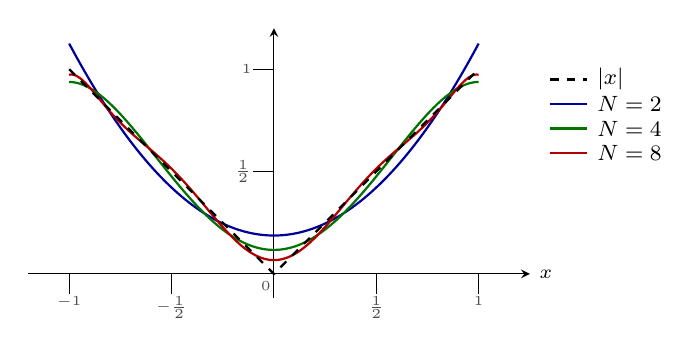
\begin{tikzpicture}[x=2.6cm,y=2.6cm]
  \draw[->] (-1.2,0) -- (1.25,0) node[right,font=\scriptsize] {$x$};
  \draw[->] (0,-0.12) -- (0,1.2);
  \draw[sig] plot coordinates {(-1.0000,1.1250) (-0.9900,1.1063) (-0.9800,1.0879) (-0.9700,1.0696) (-0.9600,1.0515) (-0.9500,1.0336) (-0.9400,1.0159) (-0.9300,0.9983) (-0.9200,0.9810) (-0.9100,0.9638) (-0.9000,0.9469) (-0.8900,0.9301) (-0.8800,0.9135) (-0.8700,0.8971) (-0.8600,0.8809) (-0.8500,0.8648) (-0.8400,0.8490) (-0.8300,0.8333) (-0.8200,0.8179) (-0.8100,0.8026) (-0.8000,0.7875) (-0.7900,0.7726) (-0.7800,0.7579) (-0.7700,0.7433) (-0.7600,0.7290) (-0.7500,0.7148) (-0.7400,0.7009) (-0.7300,0.6871) (-0.7200,0.6735) (-0.7100,0.6601) (-0.7000,0.6469) (-0.6900,0.6338) (-0.6800,0.6210) (-0.6700,0.6083) (-0.6600,0.5959) (-0.6500,0.5836) (-0.6400,0.5715) (-0.6300,0.5596) (-0.6200,0.5479) (-0.6100,0.5363) (-0.6000,0.5250) (-0.5900,0.5138) (-0.5800,0.5029) (-0.5700,0.4921) (-0.5600,0.4815) (-0.5500,0.4711) (-0.5400,0.4609) (-0.5300,0.4508) (-0.5200,0.4410) (-0.5100,0.4313) (-0.5000,0.4219) (-0.4900,0.4126) (-0.4800,0.4035) (-0.4700,0.3946) (-0.4600,0.3859) (-0.4500,0.3773) (-0.4400,0.3690) (-0.4300,0.3608) (-0.4200,0.3529) (-0.4100,0.3451) (-0.4000,0.3375) (-0.3900,0.3301) (-0.3800,0.3229) (-0.3700,0.3158) (-0.3600,0.3090) (-0.3500,0.3023) (-0.3400,0.2959) (-0.3300,0.2896) (-0.3200,0.2835) (-0.3100,0.2776) (-0.3000,0.2719) (-0.2900,0.2663) (-0.2800,0.2610) (-0.2700,0.2558) (-0.2600,0.2509) (-0.2500,0.2461) (-0.2400,0.2415) (-0.2300,0.2371) (-0.2200,0.2329) (-0.2100,0.2288) (-0.2000,0.2250) (-0.1900,0.2213) (-0.1800,0.2179) (-0.1700,0.2146) (-0.1600,0.2115) (-0.1500,0.2086) (-0.1400,0.2059) (-0.1300,0.2033) (-0.1200,0.2010) (-0.1100,0.1988) (-0.1000,0.1969) (-0.0900,0.1951) (-0.0800,0.1935) (-0.0700,0.1921) (-0.0600,0.1909) (-0.0500,0.1898) (-0.0400,0.1890) (-0.0300,0.1883) (-0.0200,0.1879) (-0.0100,0.1876) (0.0000,0.1875) (0.0100,0.1876) (0.0200,0.1879) (0.0300,0.1883) (0.0400,0.1890) (0.0500,0.1898) (0.0600,0.1909) (0.0700,0.1921) (0.0800,0.1935) (0.0900,0.1951) (0.1000,0.1969) (0.1100,0.1988) (0.1200,0.2010) (0.1300,0.2033) (0.1400,0.2059) (0.1500,0.2086) (0.1600,0.2115) (0.1700,0.2146) (0.1800,0.2179) (0.1900,0.2213) (0.2000,0.2250) (0.2100,0.2288) (0.2200,0.2329) (0.2300,0.2371) (0.2400,0.2415) (0.2500,0.2461) (0.2600,0.2509) (0.2700,0.2558) (0.2800,0.2610) (0.2900,0.2663) (0.3000,0.2719) (0.3100,0.2776) (0.3200,0.2835) (0.3300,0.2896) (0.3400,0.2959) (0.3500,0.3023) (0.3600,0.3090) (0.3700,0.3158) (0.3800,0.3229) (0.3900,0.3301) (0.4000,0.3375) (0.4100,0.3451) (0.4200,0.3529) (0.4300,0.3608) (0.4400,0.3690) (0.4500,0.3773) (0.4600,0.3859) (0.4700,0.3946) (0.4800,0.4035) (0.4900,0.4126) (0.5000,0.4219) (0.5100,0.4313) (0.5200,0.4410) (0.5300,0.4508) (0.5400,0.4609) (0.5500,0.4711) (0.5600,0.4815) (0.5700,0.4921) (0.5800,0.5029) (0.5900,0.5138) (0.6000,0.5250) (0.6100,0.5363) (0.6200,0.5479) (0.6300,0.5596) (0.6400,0.5715) (0.6500,0.5836) (0.6600,0.5959) (0.6700,0.6083) (0.6800,0.6210) (0.6900,0.6338) (0.7000,0.6469) (0.7100,0.6601) (0.7200,0.6735) (0.7300,0.6871) (0.7400,0.7009) (0.7500,0.7148) (0.7600,0.7290) (0.7700,0.7433) (0.7800,0.7579) (0.7900,0.7726) (0.8000,0.7875) (0.8100,0.8026) (0.8200,0.8179) (0.8300,0.8333) (0.8400,0.8490) (0.8500,0.8648) (0.8600,0.8809) (0.8700,0.8971) (0.8800,0.9135) (0.8900,0.9301) (0.9000,0.9469) (0.9100,0.9638) (0.9200,0.9810) (0.9300,0.9983) (0.9400,1.0159) (0.9500,1.0336) (0.9600,1.0515) (0.9700,1.0696) (0.9800,1.0879) (0.9900,1.1063) (1.0000,1.1250)};
  \draw[grn] plot coordinates {(-1.0000,0.9375) (-0.9900,0.9372) (-0.9800,0.9362) (-0.9700,0.9346) (-0.9600,0.9325) (-0.9500,0.9297) (-0.9400,0.9264) (-0.9300,0.9225) (-0.9200,0.9181) (-0.9100,0.9133) (-0.9000,0.9079) (-0.8900,0.9020) (-0.8800,0.8957) (-0.8700,0.8890) (-0.8600,0.8819) (-0.8500,0.8743) (-0.8400,0.8664) (-0.8300,0.8581) (-0.8200,0.8495) (-0.8100,0.8405) (-0.8000,0.8312) (-0.7900,0.8216) (-0.7800,0.8117) (-0.7700,0.8015) (-0.7600,0.7911) (-0.7500,0.7805) (-0.7400,0.7696) (-0.7300,0.7585) (-0.7200,0.7472) (-0.7100,0.7358) (-0.7000,0.7241) (-0.6900,0.7123) (-0.6800,0.7004) (-0.6700,0.6884) (-0.6600,0.6762) (-0.6500,0.6639) (-0.6400,0.6516) (-0.6300,0.6391) (-0.6200,0.6266) (-0.6100,0.6141) (-0.6000,0.6015) (-0.5900,0.5889) (-0.5800,0.5763) (-0.5700,0.5636) (-0.5600,0.5510) (-0.5500,0.5384) (-0.5400,0.5258) (-0.5300,0.5133) (-0.5200,0.5008) (-0.5100,0.4884) (-0.5000,0.4761) (-0.4900,0.4638) (-0.4800,0.4516) (-0.4700,0.4396) (-0.4600,0.4276) (-0.4500,0.4158) (-0.4400,0.4041) (-0.4300,0.3925) (-0.4200,0.3811) (-0.4100,0.3698) (-0.4000,0.3587) (-0.3900,0.3477) (-0.3800,0.3370) (-0.3700,0.3264) (-0.3600,0.3160) (-0.3500,0.3059) (-0.3400,0.2959) (-0.3300,0.2861) (-0.3200,0.2766) (-0.3100,0.2673) (-0.3000,0.2582) (-0.2900,0.2494) (-0.2800,0.2408) (-0.2700,0.2324) (-0.2600,0.2243) (-0.2500,0.2165) (-0.2400,0.2090) (-0.2300,0.2017) (-0.2200,0.1947) (-0.2100,0.1879) (-0.2000,0.1815) (-0.1900,0.1753) (-0.1800,0.1695) (-0.1700,0.1639) (-0.1600,0.1586) (-0.1500,0.1537) (-0.1400,0.1490) (-0.1300,0.1447) (-0.1200,0.1406) (-0.1100,0.1369) (-0.1000,0.1335) (-0.0900,0.1304) (-0.0800,0.1277) (-0.0700,0.1252) (-0.0600,0.1231) (-0.0500,0.1213) (-0.0400,0.1198) (-0.0300,0.1187) (-0.0200,0.1178) (-0.0100,0.1174) (0.0000,0.1172) (0.0100,0.1174) (0.0200,0.1178) (0.0300,0.1187) (0.0400,0.1198) (0.0500,0.1213) (0.0600,0.1231) (0.0700,0.1252) (0.0800,0.1277) (0.0900,0.1304) (0.1000,0.1335) (0.1100,0.1369) (0.1200,0.1406) (0.1300,0.1447) (0.1400,0.1490) (0.1500,0.1537) (0.1600,0.1586) (0.1700,0.1639) (0.1800,0.1695) (0.1900,0.1753) (0.2000,0.1815) (0.2100,0.1879) (0.2200,0.1947) (0.2300,0.2017) (0.2400,0.2090) (0.2500,0.2165) (0.2600,0.2243) (0.2700,0.2324) (0.2800,0.2408) (0.2900,0.2494) (0.3000,0.2582) (0.3100,0.2673) (0.3200,0.2766) (0.3300,0.2861) (0.3400,0.2959) (0.3500,0.3059) (0.3600,0.3160) (0.3700,0.3264) (0.3800,0.3370) (0.3900,0.3477) (0.4000,0.3587) (0.4100,0.3698) (0.4200,0.3811) (0.4300,0.3925) (0.4400,0.4041) (0.4500,0.4158) (0.4600,0.4276) (0.4700,0.4396) (0.4800,0.4516) (0.4900,0.4638) (0.5000,0.4761) (0.5100,0.4884) (0.5200,0.5008) (0.5300,0.5133) (0.5400,0.5258) (0.5500,0.5384) (0.5600,0.5510) (0.5700,0.5636) (0.5800,0.5763) (0.5900,0.5889) (0.6000,0.6015) (0.6100,0.6141) (0.6200,0.6266) (0.6300,0.6391) (0.6400,0.6516) (0.6500,0.6639) (0.6600,0.6762) (0.6700,0.6884) (0.6800,0.7004) (0.6900,0.7123) (0.7000,0.7241) (0.7100,0.7358) (0.7200,0.7472) (0.7300,0.7585) (0.7400,0.7696) (0.7500,0.7805) (0.7600,0.7911) (0.7700,0.8015) (0.7800,0.8117) (0.7900,0.8216) (0.8000,0.8312) (0.8100,0.8405) (0.8200,0.8495) (0.8300,0.8581) (0.8400,0.8664) (0.8500,0.8743) (0.8600,0.8819) (0.8700,0.8890) (0.8800,0.8957) (0.8900,0.9020) (0.9000,0.9079) (0.9100,0.9133) (0.9200,0.9181) (0.9300,0.9225) (0.9400,0.9264) (0.9500,0.9297) (0.9600,0.9325) (0.9700,0.9346) (0.9800,0.9362) (0.9900,0.9372) (1.0000,0.9375)};
  \draw[res] plot coordinates {(-1.0000,0.9727) (-0.9900,0.9739) (-0.9800,0.9728) (-0.9700,0.9697) (-0.9600,0.9648) (-0.9500,0.9583) (-0.9400,0.9506) (-0.9300,0.9417) (-0.9200,0.9320) (-0.9100,0.9216) (-0.9000,0.9106) (-0.8900,0.8992) (-0.8800,0.8875) (-0.8700,0.8755) (-0.8600,0.8635) (-0.8500,0.8514) (-0.8400,0.8394) (-0.8300,0.8274) (-0.8200,0.8156) (-0.8100,0.8039) (-0.8000,0.7925) (-0.7900,0.7813) (-0.7800,0.7703) (-0.7700,0.7596) (-0.7600,0.7491) (-0.7500,0.7388) (-0.7400,0.7289) (-0.7300,0.7191) (-0.7200,0.7095) (-0.7100,0.7002) (-0.7000,0.6910) (-0.6900,0.6821) (-0.6800,0.6732) (-0.6700,0.6645) (-0.6600,0.6559) (-0.6500,0.6473) (-0.6400,0.6388) (-0.6300,0.6303) (-0.6200,0.6219) (-0.6100,0.6134) (-0.6000,0.6049) (-0.5900,0.5963) (-0.5800,0.5876) (-0.5700,0.5789) (-0.5600,0.5700) (-0.5500,0.5611) (-0.5400,0.5519) (-0.5300,0.5426) (-0.5200,0.5332) (-0.5100,0.5236) (-0.5000,0.5138) (-0.4900,0.5038) (-0.4800,0.4937) (-0.4700,0.4833) (-0.4600,0.4728) (-0.4500,0.4621) (-0.4400,0.4512) (-0.4300,0.4402) (-0.4200,0.4290) (-0.4100,0.4176) (-0.4000,0.4061) (-0.3900,0.3945) (-0.3800,0.3828) (-0.3700,0.3710) (-0.3600,0.3591) (-0.3500,0.3471) (-0.3400,0.3351) (-0.3300,0.3231) (-0.3200,0.3111) (-0.3100,0.2991) (-0.3000,0.2872) (-0.2900,0.2753) (-0.2800,0.2636) (-0.2700,0.2519) (-0.2600,0.2404) (-0.2500,0.2291) (-0.2400,0.2180) (-0.2300,0.2071) (-0.2200,0.1964) (-0.2100,0.1860) (-0.2000,0.1759) (-0.1900,0.1662) (-0.1800,0.1567) (-0.1700,0.1477) (-0.1600,0.1390) (-0.1500,0.1307) (-0.1400,0.1229) (-0.1300,0.1155) (-0.1200,0.1086) (-0.1100,0.1022) (-0.1000,0.0963) (-0.0900,0.0909) (-0.0800,0.0860) (-0.0700,0.0816) (-0.0600,0.0779) (-0.0500,0.0747) (-0.0400,0.0720) (-0.0300,0.0700) (-0.0200,0.0685) (-0.0100,0.0676) (0.0000,0.0673) (0.0100,0.0676) (0.0200,0.0685) (0.0300,0.0700) (0.0400,0.0720) (0.0500,0.0747) (0.0600,0.0779) (0.0700,0.0816) (0.0800,0.0860) (0.0900,0.0909) (0.1000,0.0963) (0.1100,0.1022) (0.1200,0.1086) (0.1300,0.1155) (0.1400,0.1229) (0.1500,0.1307) (0.1600,0.1390) (0.1700,0.1477) (0.1800,0.1567) (0.1900,0.1662) (0.2000,0.1759) (0.2100,0.1860) (0.2200,0.1964) (0.2300,0.2071) (0.2400,0.2180) (0.2500,0.2291) (0.2600,0.2404) (0.2700,0.2519) (0.2800,0.2636) (0.2900,0.2753) (0.3000,0.2872) (0.3100,0.2991) (0.3200,0.3111) (0.3300,0.3231) (0.3400,0.3351) (0.3500,0.3471) (0.3600,0.3591) (0.3700,0.3710) (0.3800,0.3828) (0.3900,0.3945) (0.4000,0.4061) (0.4100,0.4176) (0.4200,0.4290) (0.4300,0.4402) (0.4400,0.4512) (0.4500,0.4621) (0.4600,0.4728) (0.4700,0.4833) (0.4800,0.4937) (0.4900,0.5038) (0.5000,0.5138) (0.5100,0.5236) (0.5200,0.5332) (0.5300,0.5426) (0.5400,0.5519) (0.5500,0.5611) (0.5600,0.5700) (0.5700,0.5789) (0.5800,0.5876) (0.5900,0.5963) (0.6000,0.6049) (0.6100,0.6134) (0.6200,0.6219) (0.6300,0.6303) (0.6400,0.6388) (0.6500,0.6473) (0.6600,0.6559) (0.6700,0.6645) (0.6800,0.6732) (0.6900,0.6821) (0.7000,0.6910) (0.7100,0.7002) (0.7200,0.7095) (0.7300,0.7191) (0.7400,0.7289) (0.7500,0.7388) (0.7600,0.7491) (0.7700,0.7596) (0.7800,0.7703) (0.7900,0.7813) (0.8000,0.7925) (0.8100,0.8039) (0.8200,0.8156) (0.8300,0.8274) (0.8400,0.8394) (0.8500,0.8514) (0.8600,0.8635) (0.8700,0.8755) (0.8800,0.8875) (0.8900,0.8992) (0.9000,0.9106) (0.9100,0.9216) (0.9200,0.9320) (0.9300,0.9417) (0.9400,0.9506) (0.9500,0.9583) (0.9600,0.9648) (0.9700,0.9697) (0.9800,0.9728) (0.9900,0.9739) (1.0000,0.9727)};
  \draw[thick,black,dashed] (-1,1) -- (0,0) -- (1,1);
  \xt{-1}{-1}\xt{-0.5}{-\frac12}\xt{0.5}{\frac12}\xt{1}{1}
  \yt{0.5}{\frac12}\yt{1}{1}
  \node[font=\tiny,gray!60!black,anchor=north east,inner sep=1pt] at (0,-0.02) {$0$};
  \begin{scope}[shift={(1.35,0.95)},font=\footnotesize]
    \draw[thick,black,dashed] (0,0) -- (0.18,0) node[right] {$|x|$};
    \draw[sig] (0,-0.12) -- (0.18,-0.12) node[right,black] {$N=2$};
    \draw[grn] (0,-0.24) -- (0.18,-0.24) node[right,black] {$N=4$};
    \draw[res] (0,-0.36) -- (0.18,-0.36) node[right,black] {$N=8$};
  \end{scope}
\end{tikzpicture}
\caption{$|x|$（黑色虚线）与勒让德多项式部分和 $\sum_{k=0}^{N}a_kP_k(x)$。$N$ 越大越贴近 $|x|$；尖角 $x=0$ 处收敛最慢。}
\end{figure}

\point{扩大适用范围。}勒让德多项式只能分解 $[-1,1]$ 上的函数。若区间是 $[-2,2]$，做自变量放缩，把 $P_n(x)$ 换成 $P_n\big(\frac x2\big)$ 即可，此时 $\int_{-2}^{2}\big[P_n(\frac x2)\big]^2\,\mathrm{d}x=\frac{4}{2n+1}$。区间不以 $0$ 为中心时再加平移：区间 $[a,b]$ 上用 $P_n\big(\frac{2x-a-b}{b-a}\big)$，正交性仍成立，自身内积为 $\frac{b-a}{2n+1}$。

%==================================================================
\section{收敛性才是最难的地方}\label{sec:conv}
上面把信号拆成正交基的整套做法，都没有涉及\textbf{收敛性}，而这恰恰是信号的正交分解最难的地方：
\begin{itemize}[nosep]
\item 一个信号拆成哈尔小波这组正交基，一定收敛吗？
\item 这组基是\textbf{完备}的吗？也就是说，任何一个 $x(t)$ 拆成它，那个等号都能打吗？
\end{itemize}
证明 $x(t)$ 可以拆成常数、$\cos$、$\sin$，用了狄利克雷三条件，推了很久才推出来（见「傅里叶级数收敛性证明」）。对每一组正交基，求系数这一套都不难，难的是收敛性。

哈尔小波和勒让德多项式的收敛性都有严格的证明。哈尔小波可以直观理解：一排一排无限拆下去，可以用阶梯函数逼近任何一个正常的函数，这与推导连续卷积公式时用阶梯函数逼近信号是同一个思路。第 \ref{sub:haar} 节的易错例子说明，少了一部分基，即使剩下的仍然两两正交，也会失去完备性。

\begin{remember}
看到「把信号拆成一组正交基的加权和」时，要关注它的收敛性（完备性）证明。
\end{remember}

%==================================================================
\section{施密特正交化}\label{sec:gs}
若有一组非正交基 $\{\alpha_k\}_{k=1\sim+\infty}$，如何变为正交基？方法叫施密特正交化(Gram--Schmidt orthogonalization)，线性代数中学过。

\begin{remember}
施密特正交化公式：
\begin{align*}
\beta_1&=\alpha_1,\\
\beta_2&=\alpha_2-\frac{\langle\alpha_2,\beta_1\rangle}{\langle\beta_1,\beta_1\rangle}\beta_1,\\
\beta_3&=\alpha_3-\frac{\langle\alpha_3,\beta_1\rangle}{\langle\beta_1,\beta_1\rangle}\beta_1-\frac{\langle\alpha_3,\beta_2\rangle}{\langle\beta_2,\beta_2\rangle}\beta_2,\\
\beta_k&=\alpha_k-\sum_{m=1}^{k-1}\frac{\langle\alpha_k,\beta_m\rangle}{\langle\beta_m,\beta_m\rangle}\beta_m .
\end{align*}
得到的 $\{\beta_k\}$ 满足 $\langle\beta_{k_1},\beta_{k_2}\rangle=0$（$k_1\ne k_2$）。
\end{remember}
每一步都是从 $\alpha_k$ 中减去它在前面各个 $\beta_m$ 上的分量（第 \ref{sec:dec} 节的 $a_m\beta_m$），剩下的部分就和前面所有的 $\beta_m$ 都正交。

\begin{figure}[H]
\centering
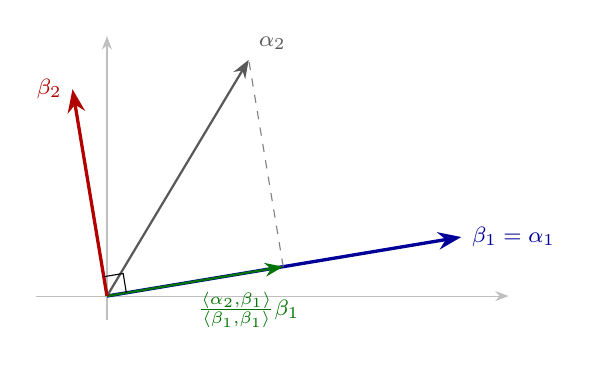
\begin{tikzpicture}[scale=1.5,>=Stealth]
  \draw[gray!50,->] (-0.6,0) -- (3.4,0);
  \draw[gray!50,->] (0,-0.2) -- (0,2.2);
  \draw[very thick,->,blue!60!black] (0,0) -- (3,0.5) node[right,font=\footnotesize] {$\beta_1=\alpha_1$};
  \draw[thick,->,gray!70!black] (0,0) -- (1.2,2) node[above right,font=\footnotesize] {$\alpha_2$};
  \draw[thick,->,green!45!black] (0,0) -- (1.4919,0.2486);
  \node[font=\footnotesize,green!45!black,anchor=north] at (1.2,0.12) {$\frac{\langle\alpha_2,\beta_1\rangle}{\langle\beta_1,\beta_1\rangle}\beta_1$};
  \draw[dashed,gray] (1.4919,0.2486) -- (1.2,2);
  \draw[very thick,->,red!70!black] (0,0) -- (-0.2919,1.7514) node[left,font=\footnotesize] {$\beta_2$};
  \draw (0.164,0.027) -- (0.137,0.191) -- (-0.027,0.164);
\end{tikzpicture}
\caption{二维示意。$\alpha_2$ 减去它在 $\beta_1$ 方向上的分量（绿），剩下的 $\beta_2$（红）与 $\beta_1$ 垂直。}
\end{figure}

\point{验证 $\langle\beta_1,\beta_2\rangle=0$。}记 $c=\frac{\langle\alpha_2,\beta_1\rangle}{\langle\beta_1,\beta_1\rangle}$，则 $\beta_2=\alpha_2-c\beta_1$。左边的 $\beta_1$ 不动，右边的数拿出来要取共轭（第 \ref{sec:ip} 节的推论）：
\begin{align*}
\langle\beta_1,\beta_2\rangle
&=\langle\beta_1,\alpha_2\rangle-\overline{c}\,\langle\beta_1,\beta_1\rangle
=\langle\beta_1,\alpha_2\rangle-\frac{\overline{\langle\alpha_2,\beta_1\rangle}}{\langle\beta_1,\beta_1\rangle}\langle\beta_1,\beta_1\rangle\\
&=\langle\beta_1,\alpha_2\rangle-\overline{\langle\alpha_2,\beta_1\rangle}
=\langle\beta_1,\alpha_2\rangle-\langle\beta_1,\alpha_2\rangle=0 .
\end{align*}
这里用到：$\langle\beta_1,\beta_1\rangle$ 是正实数，共轭等于它本身；由交换律 $\overline{\langle\alpha_2,\beta_1\rangle}=\langle\beta_1,\alpha_2\rangle$；以及 $\alpha_1=\beta_1$。实函数时所有内积都是实数，共轭可以不管。

\point{一般情形：用数学归纳法证明 $\{\beta_k\}$ 两两正交。}设 $\beta_1,\dots,\beta_{k-1}$ 已两两正交且都不为 $0$。对任意 $j<k$，按左边的叠加性、齐次性展开（左边的数拿出来不取共轭）：
\begin{align*}
\langle\beta_k,\beta_j\rangle
&=\langle\alpha_k,\beta_j\rangle-\sum_{m=1}^{k-1}\frac{\langle\alpha_k,\beta_m\rangle}{\langle\beta_m,\beta_m\rangle}\langle\beta_m,\beta_j\rangle
&&\text{（$m\ne j$ 的项 $\langle\beta_m,\beta_j\rangle=0$）}\\
&=\langle\alpha_k,\beta_j\rangle-\frac{\langle\alpha_k,\beta_j\rangle}{\langle\beta_j,\beta_j\rangle}\langle\beta_j,\beta_j\rangle=0 .
\end{align*}
所以 $\beta_k$ 与前面所有的 $\beta_j$ 正交；再由交换律，$\langle\beta_j,\beta_k\rangle=\overline{0}=0$。归纳下去，$\{\beta_k\}$ 两两正交。

\begin{note}
正交基还要求每个 $\langle\beta_k,\beta_k\rangle>0$，即 $\beta_k\ne0$。这需要 $\{\alpha_k\}$ \textbf{线性无关}（任何一个都不能由前面的线性表示），只是「每个都不为 $0$」还不够。例如 $\alpha_2=2\alpha_1$ 时，$\beta_2=2\alpha_1-2\alpha_1=0$。线性无关时，若 $\beta_k=0$，则 $\alpha_k$ 是 $\beta_1,\dots,\beta_{k-1}$（也就是 $\alpha_1,\dots,\alpha_{k-1}$）的线性组合，矛盾。得到正交基后，再按第 \ref{sec:onb} 节标准化，就是标准正交基。
\end{note}

\example{\texorpdfstring{对 $1,x,x^2$ 做施密特正交化}{对 1, x, x² 做施密特正交化}}{得到勒让德多项式}{}
在 $[-1,1]$ 上，内积 $\langle f,g\rangle=\int_{-1}^1f(x)g(x)\,\mathrm{d}x$，取 $\alpha_1=1$，$\alpha_2=x$，$\alpha_3=x^2$：
\begin{itemize}[nosep]
\item $\beta_1=1$，$\langle\beta_1,\beta_1\rangle=2$；
\item $\langle x,1\rangle=\int_{-1}^1x\,\mathrm{d}x=0$，所以 $\beta_2=x$，$\langle\beta_2,\beta_2\rangle=\frac23$；
\item $\langle x^2,1\rangle=\frac23$，$\langle x^2,x\rangle=0$，所以 $\beta_3=x^2-\frac{2/3}{2}\cdot1-0=x^2-\frac13$。
\end{itemize}
$\beta_3=\frac23\cdot\frac{3x^2-1}{2}=\frac23P_2(x)$。$\beta_1,\beta_2,\beta_3$ 与 $P_0,P_1,P_2$ 只差常数倍：对 $1,x,x^2,x^3,\dots$ 在 $[-1,1]$ 上做施密特正交化，得到的正是勒让德多项式（差一个倍数）。

%==================================================================
\section{主成分分析：从数据中学出正交基}\label{sec:pca}
主成分分析(principal component analysis，PCA)。这里只讲核心意思，不讲具体算法。以人脸识别为例。

\point{图像在计算机里是一堆数。}一幅 $M\times N$ 的彩色图像，每个像素有 R、G、B 三个数，可以看成三个矩阵；通道(channel)数 $C=3$。把它画成一个 $M\times N\times3$ 的立体矩阵，叫做张量(tensor)。

\begin{figure}[H]
\centering
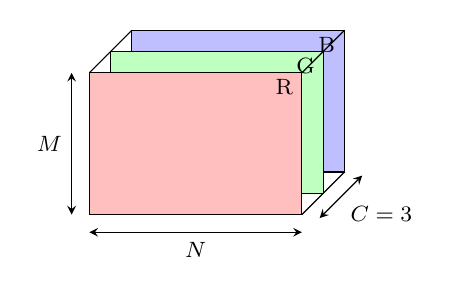
\begin{tikzpicture}[scale=0.9]
  \foreach \d/\c/\l in {0.6/blue!25/B,0.3/green!25/G,0/red!25/R}{%
    \fill[\c,draw=black] (\d,\d) rectangle ++(3,2);
    \node[font=\footnotesize] at (\d+2.75,\d+1.8) {\l};}
  \draw (0,2) -- (0.6,2.6);
  \draw (3,2) -- (3.6,2.6);
  \draw (3,0) -- (3.6,0.6);
  \draw[<->] (0,-0.25) -- (3,-0.25) node[midway,below,font=\footnotesize] {$N$};
  \draw[<->] (-0.25,0) -- (-0.25,2) node[midway,left,font=\footnotesize] {$M$};
  \draw[<->] (3.25,-0.05) -- (3.85,0.55) node[midway,below right,font=\footnotesize] {$C=3$};
\end{tikzpicture}
\caption{彩色图像是 $M\times N\times3$ 的张量：R、G、B 三个通道，每个通道一个 $M\times N$ 矩阵。}
\end{figure}

\begin{remember}
PCA 的核心：从一大堆数据中，自动地训练出一组正交基。
\end{remember}

\point{平均脸与正交基。}设有一堆人脸 $X_i$（$i=1,\dots,N$），每个 $X_i$ 都是 $M\times N\times3$ 的张量。
\begin{itemize}[nosep]
\item $A_0=\dfrac1N\sum_{i=1}^{N}X_i$，叫做\textbf{平均脸}；
\item $A_1,A_2,A_3,\dots$ 由 PCA 训练得到，满足 $\langle A_i,A_j\rangle=0$（$i\ne j$），内积为所有像素、所有通道对应相乘再相加：
\[
\langle A_i,A_j\rangle=\sum_{u=1}^{M}\sum_{v=1}^{N}\sum_{c=1}^{3}A_i(u,v,c)\,A_j(u,v,c).
\]
（像素值都是实数，共轭可以不写。）它们按特征值(eigenvalue)由大到小排列，是数据的特征向量(eigenvector)，用于人脸时又叫\textbf{特征脸}(eigenfaces)。
\end{itemize}

\point{分解一张新的人脸。}对一张新的人脸 $X$：
\[
X=a_0A_0+a_1A_1+a_2A_2+\cdots,\qquad a_k=\frac{\langle X,A_k\rangle}{\langle A_k,A_k\rangle}\quad(k=1\sim+\infty).
\]
这就是第 \ref{sec:dec} 节的公式。例如某张脸 $A=A_0+3559A_1+351A_2-256A_3+\cdots$，得到一组数 $(3559,351,-256,\dots)$，用这组数来表达图像的本质特征，并用于对图像的进一步处理（压缩、识别）。

\begin{note}
严格地说，平均脸 $A_0$ 一般与 $A_1,A_2,\dots$ 不正交，所以 $A_0$ 的系数取 $1$，其余系数要先减去平均脸再算：
\[
X=A_0+\sum_{k\ge1}a_kA_k,\qquad a_k=\frac{\langle X-A_0,A_k\rangle}{\langle A_k,A_k\rangle}.
\]
上面例子中 $A_0$ 前面的系数正是 $1$。直接用 $\langle X,A_k\rangle$ 会多出 $\frac{\langle A_0,A_k\rangle}{\langle A_k,A_k\rangle}$ 一项（用随机数据做数值试验，平均向量与前几个特征向量的内积分别约为 $-4.4$、$-2.6$、$-0.16$，都不为 $0$）。
\end{note}

\point{应用一：任何人脸都是几百张脸的线性组合。}在深度学习出现之前，这是人脸识别的标准流程。人脸识别领域曾流传一句话：世界上任何一个人的脸，都可以用 $500$ 张脸（取前 $500$ 个正交基）线性组合出来。这样的加法能反映大部分情况，至今仍在使用。

\point{应用二：照片生成相像的卡通形象。}先算出约 $500$ 个人脸正交基，同时为每个正交基准备一个对应的卡通形象「正交基」。拍一张照片，求出它在人脸正交基上的系数，再把这些系数原封不动地用到卡通形象的正交基上，就得到一张与自己比较像的卡通脸。较简单的人脸合成至今仍用这种方法；更复杂、更真实的合成现在多用深度学习。

\point{应用三：人脸识别。}识别人脸就是衡量两张脸有多相似。
\begin{itemize}[nosep]
\item 直接比像素：用 $\|X_A-X_B\|^2$ 衡量 A、B 两张脸的差异。它精确到每一个像素的差距，过于敏感，效果往往不好。
\item 比系数：把 $X_A$、$X_B$ 都分解成 $500$ 个系数，比较这 $500$ 个数之间的差距。一般比直接比像素好很多。
\end{itemize}
特征脸为什么好用：图中亮的地方像素值大、暗的地方像素值小。第一张特征脸强调脸颊、鼻子和眼睛，两个人这些部位相似，第一个系数就接近；另一张强调眉毛、眼睛、鼻子和嘴的一部分，等等。PCA 学习后会自动强调人的各种五官的组合——并没有规定「按五官识别」，它自己发现五官是人与人差别最大的地方。

\point{识别结果。}数据库 XM2VTS：$295$ 人，每人 $8$ 张照片，分四次拍摄，每次两张，每次间隔一个月。用前两次拍摄的 $4$ 张照片训练，后两次拍摄的 $4$ 张照片测试，取前 $100$ 维 PCA 进行识别：
\begin{center}
\begin{tabular}{lcc}
\toprule
 & 最近邻法 & SVM\\
\midrule
识别率 & $76.02\%$ & $80.25\%$\\
\bottomrule
\end{tabular}
\end{center}
两种方法都在 $100$ 维 PCA 系数上做识别：最近邻法(nearest neighbor)取系数之间距离最小的训练样本作为结果；支持向量机(support vector machine，SVM)是另一种分类器，识别率高一些。

\end{document}
